%
\documentclass[a4paper,10pt,fleqn]{article} % Definiert Papier = A4;
                                            % Schriftgrösse = 10Punkte;
                                            % Mathe.-Gl. Modus = linksbündig
                                            % (siehe http://lefti.amigager.de/latex/Aufbau.html)

\usepackage[utf8x]{inputenc}                % utf8x kann alle Textcodierungen interpretieren
\usepackage[T1]{fontenc} %Schriftcodierung mit UTF-8
\usepackage{textcomp} %Erweiterung von fontenc
\usepackage{lmodern} %Erweiterung des Zeichensatzes

\usepackage{graphics}                       % Package für Einfügen/Anpassen von Grafiken
\usepackage{graphicx}
\usepackage{wrapfig}                        % Package zum Einfügen von Textumflossenen Bilder

\usepackage[english,ngerman]{babel}         % ngerman = Neues Deutsch; babel = internationalisierung einschalten
\usepackage[babel,german=quotes]{csquotes}  % Deutsche Gänsefüssechen

\usepackage{hyperref}

\usepackage{amsmath}                        
\usepackage[all]{xy}
%\usepackage[xindy]{glossaries}
\usepackage{makeidx}
\usepackage{pdfpages}
\usepackage{graphicx}
\usepackage{printlen}

\usepackage{blindtext}
\usepackage{lipsum}

\usepackage{multicol}

\usepackage{multirow}

\usepackage{verbatim}

\usepackage{color}

\usepackage{eurosym}

%\usepackage{hyperref}
\usepackage{acronym}

\usepackage{enumitem}

\usepackage{setspace}

\usepackage{threeparttable} %benötigt um Fussnoten in einer Tabelle zu machen
\usepackage{longtable}


\usepackage{spreadtab} %benötigt um in Tabellen zu rechnen
\usepackage{numprint}

%Package damit eine Seite quer genommen werden kann
\usepackage{lscape}

%Damit man eine Zelle farbig markiert werden
\usepackage{colortbl}


%
% Rechnen in Tabellen. Zeichen für den Dezimalpunkt
%
\STsetdecimalsep{{.}}

\definecolor{darkgreen}{rgb}{0,0.6,0}
\usepackage{listings}
\lstset{language=[LaTeX]TeX}
\lstloadlanguages{TeX}
\lstset{basicstyle=\ttfamily\footnotesize,
        numbers=left,
        numberstyle=\tiny,
        numbersep=5pt,
        breaklines=true,
        texcsstyle=\color{black},
        backgroundcolor=\color{gray!10},
        %commentstyle=\color{darkgreen},
        %keywordstyle=\color{red}\bfseries,
        %stringstyle=\color{blue}\bfseries,
        frame=single,
        tabsize=2,
        rulecolor=\color{black!30},
        title=\lstname,
        escapeinside={\%*}{*)},
        breaklines=true,
        breakatwhitespace=true,
        framextopmargin=2pt,
        framexbottommargin=2pt,
        inputencoding=utf8x,
        extendedchars=true,
        literate={Ö}{{\"O}}1
                 {Ä}{{\"A}}1
                 {Ü}{{\"U}}1
                 {ü}{{\"u}}1
                 {ä}{{\"a}}1
                 {ö}{{\"o}}1 
       }
%
% hypersetup etwas genauer
%
\hypersetup{pdftex=true,
            hyperfigures=true,
            hyperindex=true,
            bookmarks=true,
            bookmarksopen=true,
            bookmarksnumbered=true,
            %pdfborder={0 0 0},
            hypertexnames=true,
            colorlinks=true,
            pagebackref=false,
            linktocpage=false,% link "`behing"'
            plainpages=false,
            linkcolor=black,%blue,
            %anchorcolor=black,% Color for anchor text.
            citecolor=black,%green,%Color for bibliographical citations in text.
            filecolor=black,%magenta,%Color for URLs which open local files.
            menucolor=black,%red,%Color for Acrobat menu items. pagecolor color red Color for links to other pages, but currently unused
            urlcolor=black,%red,
            pdfstartview=Fit,
            pdfview={XYZ null null null},
            pdfpagelabels,
            pageanchor=true,
            hypertexnames=false
           }
%
% hypersetup etwas rudimentärer
%
%{
    %colorlinks,
    %citecolor=black,
    %filecolor=black,
    %linkcolor=black,
    %urlcolor=black
%}

\usepackage{url}

\usepackage{cite}
\usepackage{apacite}

\usepackage{pdfpages}                        % Packet für PDF Dateimanipulation laden

\usepackage{fancyhdr}                        % http://en.wikibooks.org/wiki/LaTeX/Page_Layout#Customising_with_fancyhdr

\usepackage{siunitx}                         % benötigt um Tabellen nach einem . auszurichten


\bibliographystyle{apacite}


\pagestyle{fancy} %eigener Seitenstil
\fancyhf{} %alle Kopf- und Fusszeilenfelder bereinigen

\addtolength{\textwidth}{1.5cm}
\addtolength{\evensidemargin}{-5mm}
\addtolength{\oddsidemargin}{-5mm}

\addtolength{\headwidth}{1.5cm}

%\rhead{\setlength{\unitlength}{1mm}
%\begin{picture}(-2,7)
%    \includegraphics[width=35mm]{hslu_logo2.PNG}
%\end{picture}}

\fancyhead[L]{Projektarbeit: Autonomer Ballwerfer} %Kopfzeile links
\fancyhead[C]{} %zentrierte Kopfzeile
\fancyhead[R]{HSLU - T\&A}
%\fancyhead[R]{\includegraphics[scale=0.25]{hslu_logo2.PNG}}
\renewcommand{\headrulewidth}{0.4pt} % obere Trennlinie
\fancyfoot[L]{PREN Team 32}
\fancyfoot[C]{HS - 2014}
\fancyfoot[R]{\thepage}
\renewcommand{\footrulewidth}{0.4pt} % untere Trennlinie

%
% Anpassung der Darstellung des Literaturverzeichnis
%
\let\oldbibliography\thebibliography
\renewcommand{\thebibliography}[1]{%
  \oldbibliography{#1}%
  \setlength{\itemsep}{10pt}%
}
%
% Abbildungen und Tabellen nur mit Kurzform angeben
%
\addto\captionsngerman{
\renewcommand{\figurename}{Abb.}
\renewcommand{\tablename}{Tab.}
}
%
% Benötigt um von zwei Stellen im Text auf dieselbe Fusszeile zu referenzieren
%
\newcommand{\footnoteremember}[2]{%
  \footnote{#2\label{#1}}
  \newcounter{#1}
  \setcounter{#1}{\value{footnote}}
}
\newcommand{\footnoterecall}[1]{%
  \hyperref[#1]{\footnotemark[\value{#1}]}
} 
\makeatletter
\providecommand{\rowno}[1][__empty__]
{%
  \ifthenelse{\isundefined{\c@rowno}}
  {%
    \newcounter{rowno}
  }
  {}%
  	\ifthenelse{\equal{#1}{__empty__}}
 	 {%
       \stepcounter{rowno}%
     }
     {%
 	   \setcounter{rowno}{#1}%
     }%
  \therowno%
}
\makeatother
%
%\makeglossaries
%\include{wa/wa_glossar}
%
\documentclass[a4paper,10pt,fleqn]{article} % Definiert Papier = A4;
                                            % Schriftgrösse = 10Punkte;
                                            % Mathe.-Gl. Modus = linksbündig
                                            % (siehe http://lefti.amigager.de/latex/Aufbau.html)

\usepackage{common/Layout}
\newcommand{\myTitel}{Anhang zur Schlussdokumentation}
\newcommand{\myDokumentTyp}{Anhangsdokument}
\begin{document}
    %
    % Deck- und Titelblatt
    %
    \begin{titlepage}
    \begin{center}     
        \parindent0pt{\Huge PREN 1}\\
        \vspace*{1.2cm}
        Yves Studer\\
        Thomas Wiss\\
        Livio Kunz\\
        Nikolaus Manser\\
        MatteoTrachsel\\
        Güdel Manuel\\
        Pascal Roth\\
        \vspace*{1.2cm}
        {\Huge \myTitel}\\
        \vspace*{1cm}
%        \begin{figure*}[h!]
%            \centering
%            \includegraphics[width=0.7\textwidth]{Sourcen/Bilder/WuerfelTitel}
%        \end{figure*}
        \vspace*{10cm}
        {\normalsize Hochschule Luzern - Technik \& Architektur}\\
        {\normalsize PREN 1}\\
        \vspace*{0.6cm}
        {\normalsize Horw, Hochschule Luzern - T\&A, \today}\\
    \end{center}
\end{titlepage}

    \begin{titlepage}
    \parindent0pt {\Huge PREN 1}\\
    \vspace*{0.7cm}
    \newline
    \begin{tabular}{ p{6cm} p{5cm}}
        Yves Studer                & Thomas Wiss \\
        Dorfstrasse 28             & Bachhüsliweg 4a \\
        6264 Pfaffnau              & 6042 Dietwil \\
        +41 79 705 48 88           & +41 79 604 93 61 \\
        yves.studer@stud.hslu.ch   & thomas.wiss@stud.hslu.ch \\
                                   & \\
        Livio Kunz                 & Niklaus Manser \\
        Hubelmatt 7                 & Brunnmattstrasse 11\\
        6206 Neuenkirch         & 6010 Kriens \\
        +41 79 811 53 03           & +41 77 405 58 56 \\
        livio.kunz@stud.hslu.ch    & niklaus.manser@stud.hslu.ch \\
                                   & \\
        Matteo Trachsel			   & Manuel Güdel \\
        Hofstrasse 4               & Riedtalstrasse 4\\
        6004 Luzern                & 4800 Zofingen\\
        +41 79 511 57 88           & +41 79 774 41 40 \\
        matteo.trachsel@stud.hslu.ch & manuel.guedel@stud.hslu.ch \\
        						   & \\
        Pascal Roth			       & \\
        Dorfstrasse 18			   & \\
        6275 Ballwil		       & \\
        +41 79 717 68 94	       & \\
        pascal.roth@stud.hslu.ch   & \\
    \end{tabular}
    \vspace*{1.7cm}
    \newline
    {\Huge Meilenstein 1 Dokumentation}\\
    \vspace*{1.2cm}\\
    {\normalsize Dozent: Markus Thalmann}\\
    \vspace*{0.2cm}\\
    {\normalsize Hochschule Luzern - Technik \& Architektur}\\
    {\normalsize Interdisziplinäre Projekarbeit 2014}\\
    \vspace*{2.3cm}
    \newline
    {\normalsize Horw, Hochschule Luzern - T\&A, \today}\\
\end{titlepage}

    %
    % Inhaltsverzeichnis umbenennen und anschliessend einen Seitenumbruch
    % 
    \renewcommand{\contentsname}{Inhalt}
    \tableofcontents
    \newpage
    


    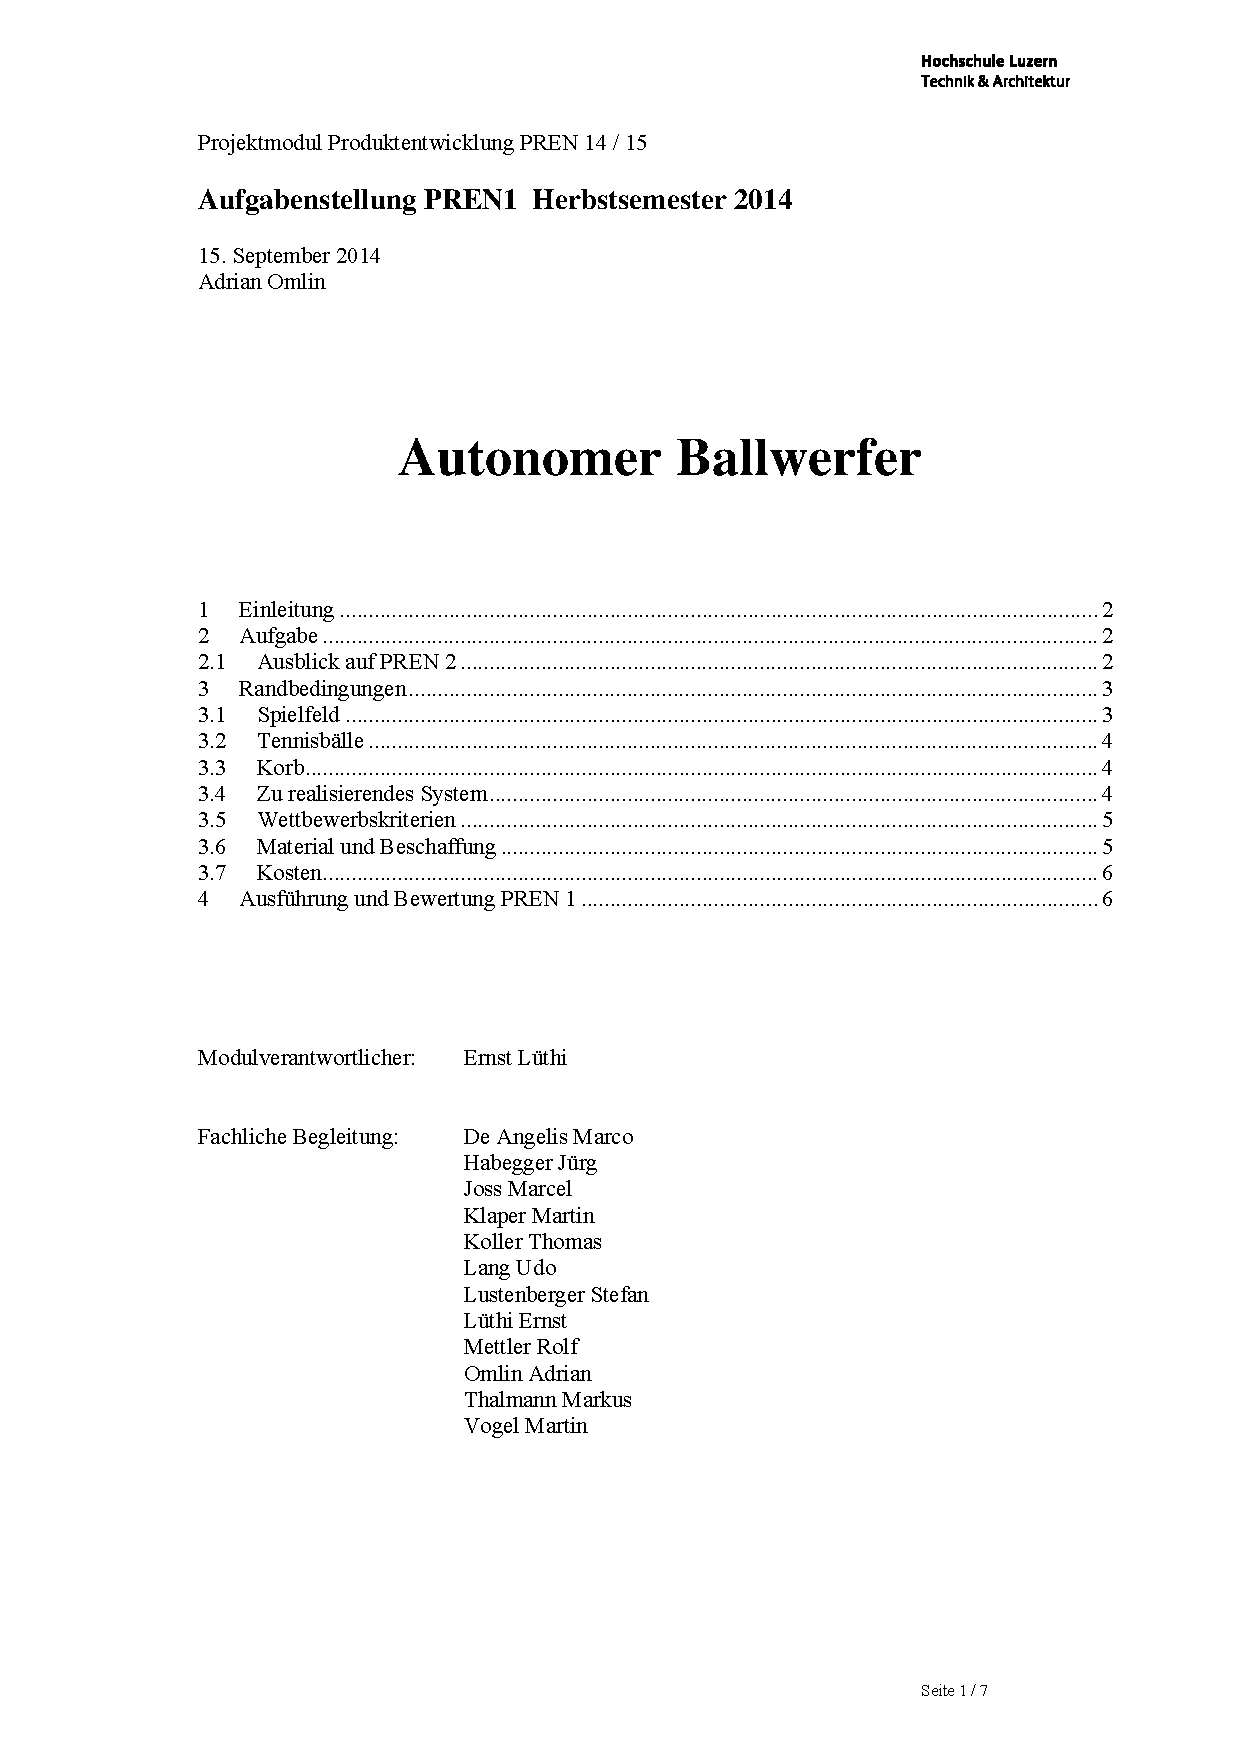
\includepdf[page=1 , offset=0cm -1.9cm, width=1\textwidth,picturecommand={\centering},pagecommand=\section{Aufgabenstellung}{\thispagestyle{fancy}},]{Anhangsdokument/Aufgabenstellung_PREN1_H14.pdf}
    
    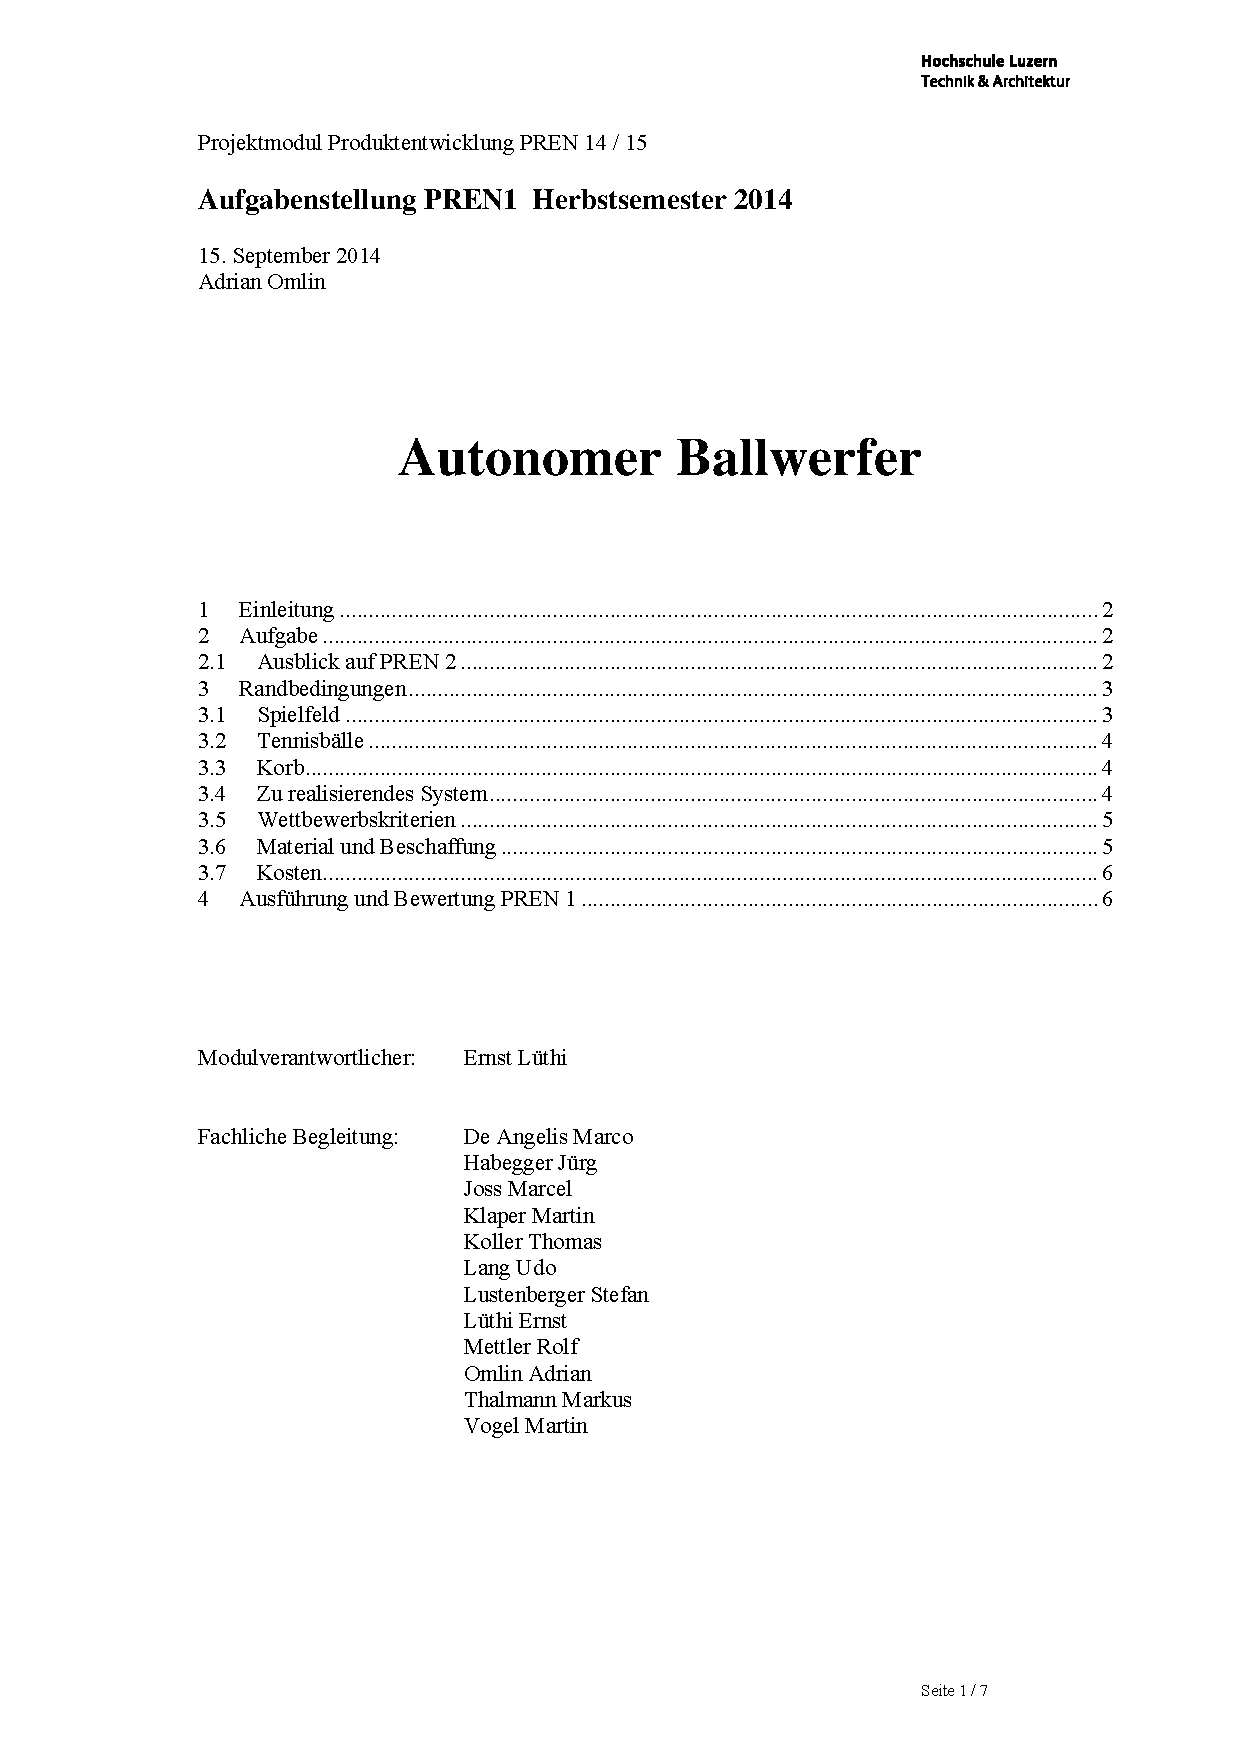
\includepdf[page=2- , offset=0cm -1.35cm, width=1\textwidth,picturecommand={\centering},pagecommand={\thispagestyle{fancy}},]{Anhangsdokument/Aufgabenstellung_PREN1_H14.pdf}
     
     \begin{landscape}
     	\section{Risikokatalog}
			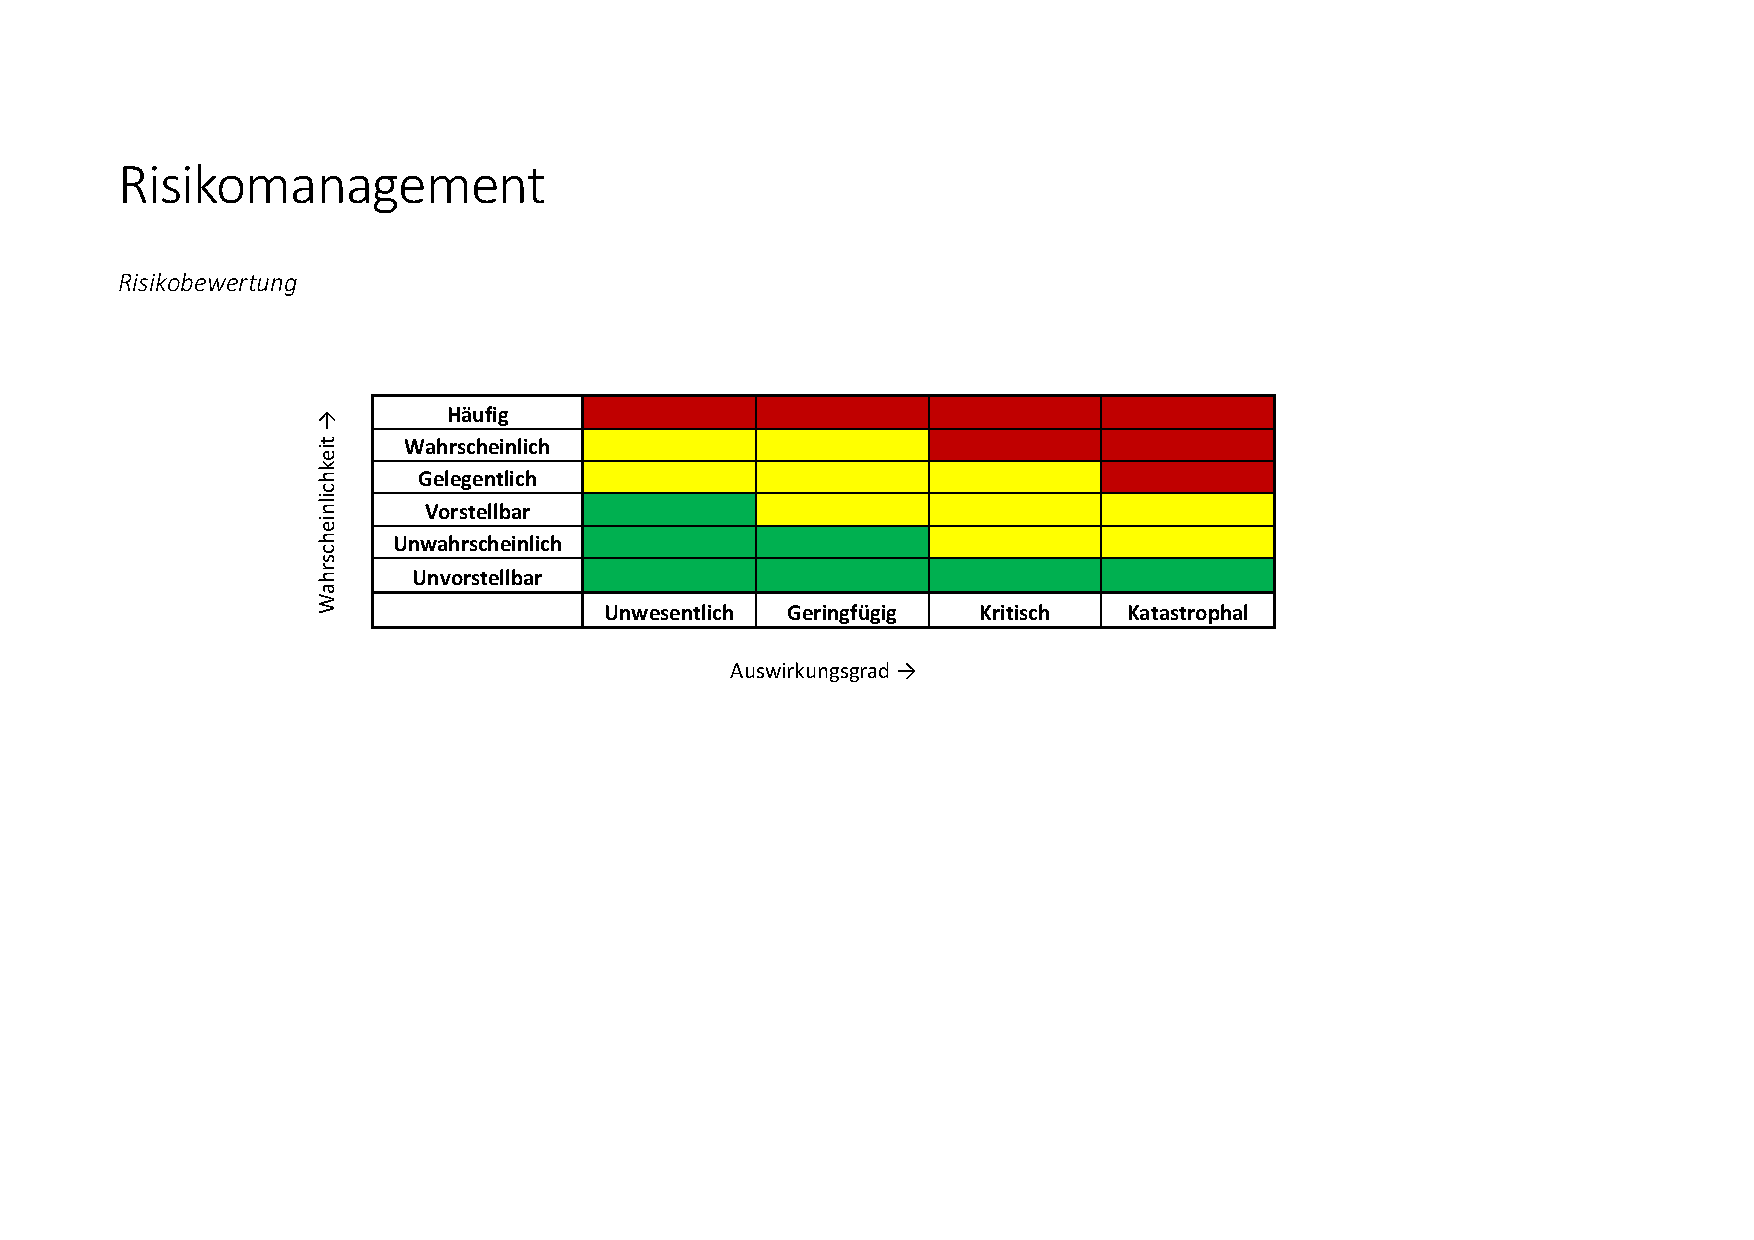
\includegraphics[page=1,scale=0.73,clip,trim=17mm 27mm 31mm 39mm]{Anhangsdokument/Risikomanagement.pdf}
			\newpage  			
			\includegraphics[page=2,scale=1,clip,trim=20mm 22mm 21mm 32mm]{Anhangsdokument/Risikomanagement.pdf}
			\newpage  			
			\includegraphics[page=3,scale=1,clip,trim=20mm 22mm 21mm 22mm]{Anhangsdokument/Risikomanagement.pdf}
			\newpage  			
			\includegraphics[page=4,scale=1,clip,trim=20mm 22mm 21mm 22mm]{Anhangsdokument/Risikomanagement.pdf}
			\newpage  			
			\includegraphics[page=5,scale=1,clip,trim=20mm 22mm 21mm 22mm]{Anhangsdokument/Risikomanagement.pdf}	
     \end{landscape} 
     
     
  	 \begin{landscape}
	\section{Recherche-Tabelle}	
		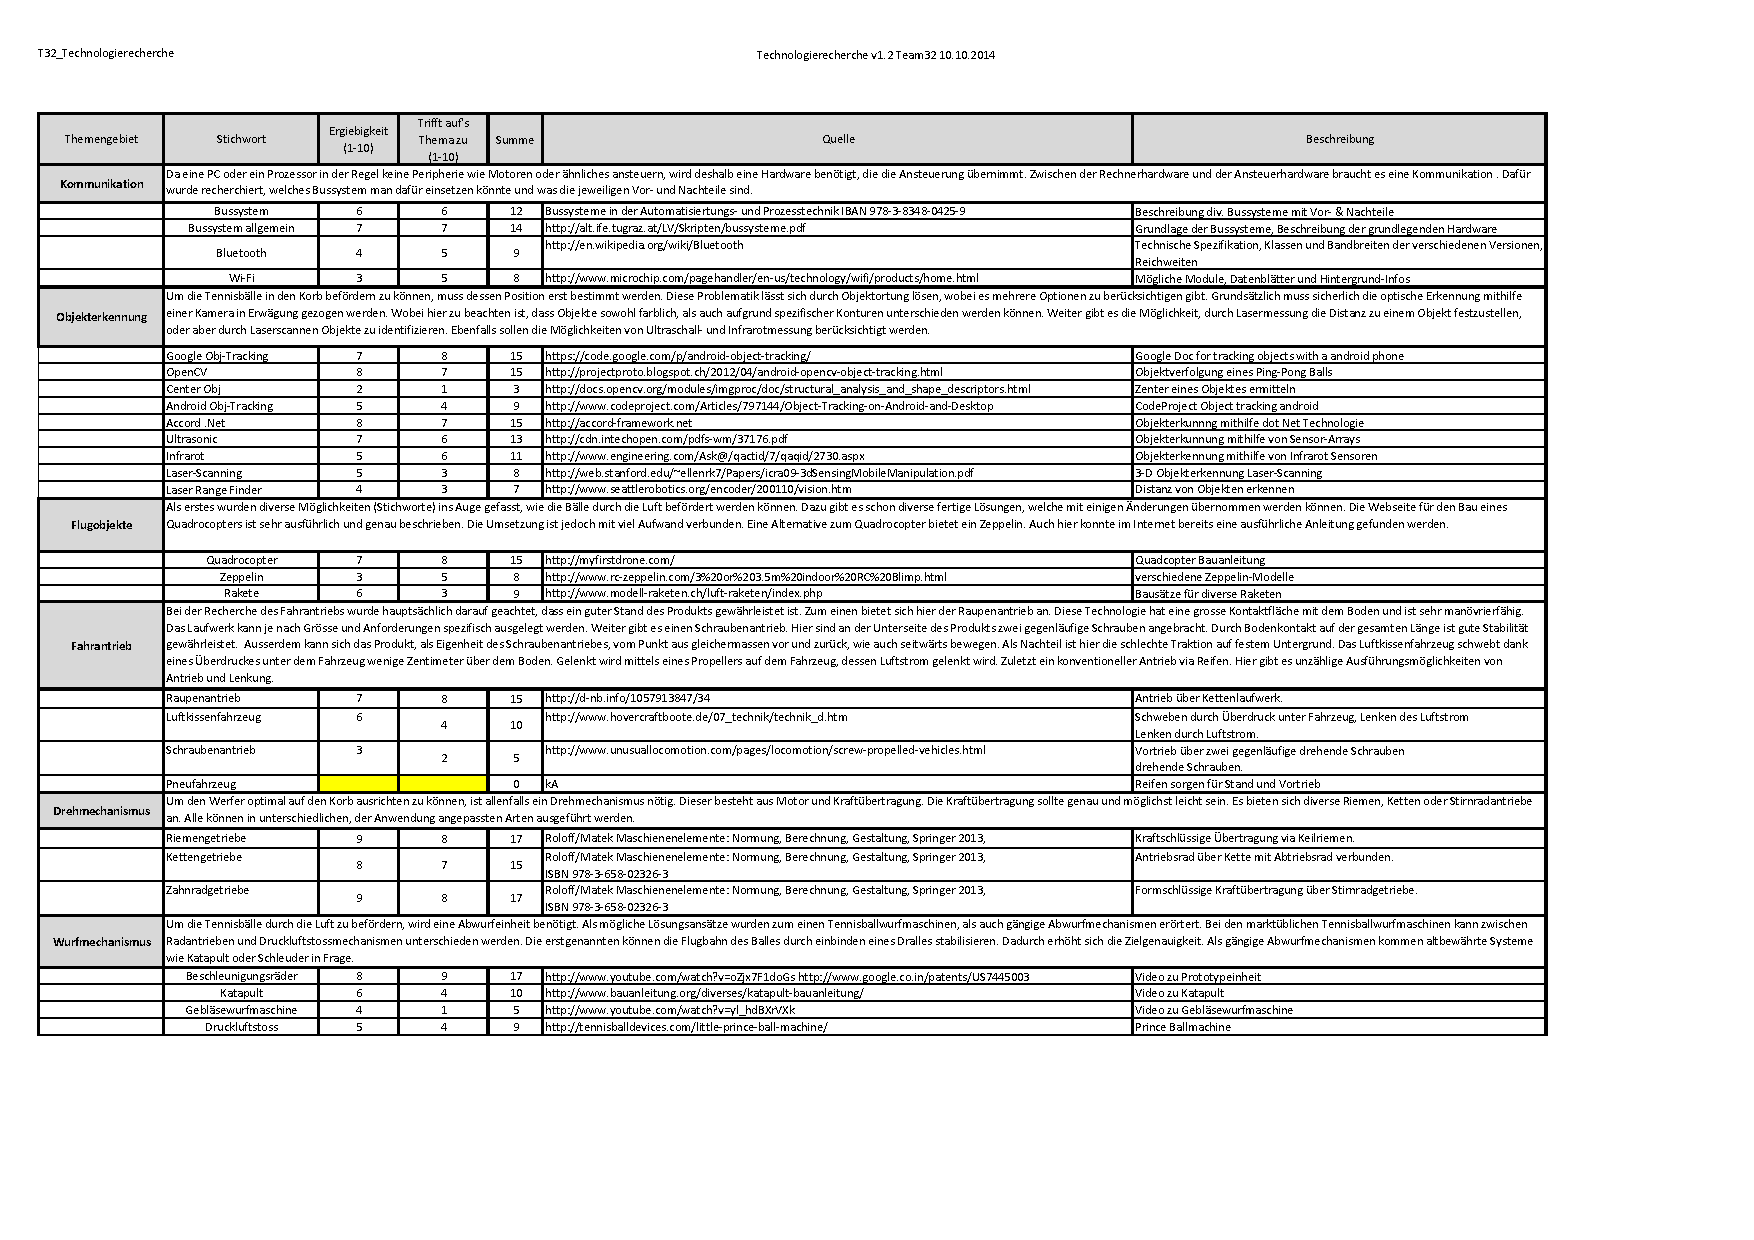
\includegraphics[page=1,scale=0.84,clip,trim=6.4mm 39mm 35mm 18mm]{Recherche/Extern/Produktrecherche.pdf}
		\newpage
		\includegraphics[page=2,scale=0.82,clip,trim=6.4mm 39mm 35mm 18mm]{Recherche/Extern/Produktrecherche.pdf}
\end{landscape} 
  	 \section{Kommunikation}
In diesem Abschnitt werden zwei Problembereiche angeschnitten. Zum einen kann ein PC oder ein Prozessor keine Peripherie (Motoren, Wurfmechanismus etc.) ansteuern, weshalb Hardware benötigt wird, welche die Ansteuerung übernimmt. Zwischen der Rechnerhardware und der Ansteuerhardware bedarf es einer Kommunikationsschnittstelle. Dafür wurde recherchiert, welches Bussystem man dafür einsetzen könnte und was die jeweiligen Vor- und Nachteile sind. Des weiteren muss für die kabellose Übermittlung des Startsignals eine geeignete Lösung gefunden werden.

\subsection{USB}
Der Universal Serial Bus ist eine gängige kabelgebundene serielle Schnittstelle, mit der Daten von einem Host an ein oder mehrere Slaves\footnote{Peripherie-Geräte} zu übertragen. Die Übertragung findet differentiell statt, was eine gute Störunempfindlichkeit mit sich bringt. Es können Datenraten von 1.5 $\frac{Mbit}{s}$ bis zu 10 $\frac{Gbit}{s}$ realisiert werden. Der Aufbau des Systems bedingt, dass ein Master-Controller eingesetzt wird. Dies ist bei PC's standardmässig vorhanden, was bei anderen Geräten problematisch sein kann. So gibt es zum Beispiel Mobile-Phones, die nur über eine Slave-Hardware verfügen. Weiter bietet der USB-Standard diverse mechanische Formen und Grössen eines Steckers.

\subsection{Wi-Fi}
IEEE 802.11 auch Wi-Fi genannt, bezeichnet ein Standard, um Daten kabellos zwischen meinst mobilen Geräte auszutauschen. Dabei wird ein Frequenzband im 2.4 GHz oder 5 GHz Bereich verwednet. Die Bandbreite beträgt je nach Standard zwischen 2 $\frac{Mbit}{s}$ und 6.7 $\frac{Gbit}{s}$. Die Reichweite beträgt zwischen 35 m bis 100 m. Wie aus dem Modul PRG2 bekannt ist, sind die Broadcast-Übermittlungen im HSLU-Netz gesperrt. Dies erschwert die Erstellung einer Datenverbindung, da die dynamisch vergebenen IP-Adressen benötigt werden.

\subsection{Bluetooth}
Dies ist ein Standard, mit dessen Hilfe Daten zwischen Geräten ausgetauscht werden können. Wie Wi-Fi verwendet auch Bluetooth das 2.4 GHz Frequenzband. Die Bandbreite beträgt je nach Version zwischen 1 $\frac{Mbit}{s}$ und 4 $\frac{Mbit}{s}$. Die Reichweite beträgt je nach Klasse zwischen 1m bis 100 m. Bluetooth verwendet ein Frequenzsprungverfahren, um allfälligen Störungen durch andere Geräte zu entgehen. 
  	 \subsection{Object-Tracking – Objekt Verfolgung}
\subsubsection{Google Obj-Tracking}
Es wird mithilfe einer Android Smartphone, dessen Kamera und einem Adruino Uno Controller ein Objekt verfolgt. Dazu läuft auf dem Android Smartphone eine App die mithilfe der Kamera die Objekterkennung durchführt und die Informationen an den Controller weitergibt. Es ist eine Anleitung und Source Code vorhanden.

\subsubsection{OpenCV}
OpenCV ist eine OpenSource Bibliothek die eine Vielzahl von Bildverarbeitungsalgorithmen bereitstellt. Es wird beschrieben wie mithilfe von OpenCV und einer Android Kamera ein Objekt erkannt werden kann. Vorhanden sind Code Beispiele und Tutorials.

\subsubsection{Center an Object}
Code Beispiele wie man ein Objekt einmitten kann mithilfe von OpenCV. Code Beispiele sind in C++ und Python gegeben.

\subsubsection{Android Obj-Tracking}
Ein Tutorial für Object Tracking mit BoofCV. BoofCV ist eine Open-Source Bibliothek für Java. Hat Code Beispiele und Erklärungen wie man ein Objekt verfolgen kann.

\subsubsection{Accord.Net}
Accord.Net ist eine OpenSource Bibliothek für das .Net Framework. Es werden Code Beispiele angeboten und Tutorials
	
\subsubsection{Ultrasonic}
Beschreibt wie die Erkennung von Objekten mithilfe von Ultraschallsensoren.

\subsubsection{Infrarot}
Infrarot Sensoren geben einen Infrarot Lichtstrahl ab, ein Sensor erkennt dann die Rückstrahlung womit sich Objekte erkennen lassen. 

\subsubsection{Laser-Scanning}
Mithilfe eines Lasers können 3-D Modelle einer Umgebung erstellt werden indem viele Messungen durchgeführt werden und dann die einzelnen Punkte zu einem Gebilde zusammengesetzt werden.

\subsubsection{Laser-Range-Finder}
Laser Range Finder (LRF) können sehr gut dazu eingesetzt werden Distanzen zu bestimmen. Es werden die verschiedenen 

  
  	 \subsection{Flugobjekte}
Als Flugobjekte wurden drei verschiedene Möglichkeiten ins Auge gefasst. Dazu zählt ein Quadcopter, eine Zeppelin und eine Rakete. Die Hauptschwierigkeit besteht bei der Steuerung der Objekte in der Flugphase. Eine weitere Teilschwierigkeit ist, eine berechenbare Flugbahn zu erreichen. 

\subsubsection{Quadrocopter}
\textbf{Vorteile}\\
Ein Quadrocopter kann als fertiger Baukasten gekaut und zusammengebaut werden. Die Flugsteuerung erfolgt über eine fertige Software.\\
\\
\textbf{Nachteile}\\
Die Steuerung des Quadrocopter ist sehr schwierig. Die Orientierung im Raum ist mit einer einfachen Software nicht möglich. Um eine bestimmte Flugbahn einzuhalten, brauchte man diverse Kameras, welche im Raum verteilt sind. Der ganze Quadrocopter und die Steuerung sind sehr kostenintensiv.\\
\\
\textbf{Umsetzbarkeit}\\
Eine Möglichkeit, für eine effiziente Umsetzung eines Quadrocopters in das Konzept ist fast 
Unmöglich. Die Kosten werden bei weitem überschritten. Die genaue Steuerung im Raum ist extrem schwierig. 

\subsubsection{Zeppelin}
\textbf{Vorteile}\\
Der Zeppelin kann als fertiger Baukasten gekauft werden. Die Modelle können der jeweiligen Hebelast angepasst werden. \\
\\
\textbf{Nachteile}\\
Der Auftriebskörper für eine kleine Masse zu heben, ist sehr gross. Die Steuerung des ganzen Zeppelins verläuft sehr träge.\\
\\
\textbf{Umsetzbarkeit}\\
Aus Platzgründen, welcher der Auftriebkörper benötigt, ist der Zeppelin sehr schwierig zu realisieren. \\
\\
\subsubsection{Rakete}
\textbf{Vorteile}\\
Sehr schneller Vortrieb des Wurfskörpers.\\
\\
\textbf{Nachteile}\\
Die Wurfbahn einer Rakete auf kleine Distanz ist fast unmöglich. \\
\\
\textbf{Umsetzbarkeit}\\
Die Umsetzung eines Raketenantriebes ist unmöglich.\\
\\
\\
Als erstes wurden diverse ins Auge gefasst, wie die Bälle durch die Luft befördert werden können. Dazu gibt es schon diverse fertige Lösungen, welche mit einigen Änderungen übernommen werden können. Die Webseite für den Bau eines Quadrocopters ist sehr ausführlich und genau beschrieben. Die Umsetzung ist jedoch mit viel Aufwand verbunden. Eine Alternative zum Quadrocopter bietet ein Zeppelin. Auch hier konnte im Internet bereits eine ausführliche Anleitung gefunden werden.
 
  	 \subsection{Fahrantrieb}
Bei der Recherche des Fahrantriebs wurde hauptsächlich darauf geachtet, dass ein guter Stand des Produkts gewährleistet ist. Zum einen bietet sich hier der Raupenantrieb an. Diese Technologie hat eine grosse Kontaktfläche mit dem Boden und ist sehr manövrierfähig. Das Laufwerk kann je nach Grösse und Anforderungen spezifisch ausgelegt werden. Weiter gibt es einen Schraubenantrieb. Hier sind an der Unterseite des Produkts zwei gegenläufige Schrauben angebracht. Durch Bodenkontakt auf der gesamten Länge ist gute Stabilität gewährleistet.  Ausserdem kann sich das Produkt, als Eigenheit des Schraubenantriebes, vom Punkt aus gleichermassen vor und zurück, wie auch seitwärts bewegen. Als Nachteil ist hier die schlechte Traktion auf festem Untergrund. Das Luftkissenfahrzeug schwebt dank eines Überdruckes unter dem Fahrzeug wenige Zentimeter über dem Boden. Gelenkt wird mittels eines Propellers auf dem Fahrzeug, dessen Luftstrom gelenkt wird. Zuletzt ein konventioneller Antrieb via Reifen. Hier gibt es unzählige Ausführungsmöglichkeiten von Antrieb und Lenkung. 
   
  	 \section{Drehmechanismus}
Falls der Werfer keine seitlichen Bewegungen ausführen kann, muss er sich mithilfe eines Drehmechanismus auf den Korb einstellen können. Diese Drehung kann auf verschiedene Weise realisiert werden. Die Anforderung ist, dass sich der Werfer bei Bedarf in einem bestimmten Winkelbereich nach links und rechts bewegen kann. Angetrieben von einem Elektromotor muss diese Verdrehung so präzise sein, dass ein exakter Wurf möglich ist. Weiter spielt nach den Produkteanforderungen auch die Geschwindigkeit der jeweiligen Verschiebung eine Rolle. Die gewählte Art der Kraftübertragung muss demnach geringe Trägheit aufweisen und kleine aber schnelle Bewegungen ermöglichen. 
 
\subsection{Riemengetriebe}
Bei Riemengetrieben wird die zu übertragende Kraft formschlüssig oder kraftschlüssig mit einem Zugmittel übertragen. Als kraftschlüssig übertragende Zugmittel werden Flach-, Keil- und Keilrippenriemen eingesetzt. Demgegenüber sind die Synchronriemen (Zahnriemen), die formschlüssig übertragen. \\
Ein grosser Vorteil dieser Technologie ist, dass sie in allen erdenklichen Lagen eingesetzt werden kann. Auch können mit nur einer Getriebestufe sehr grosse Übersetzungen erreicht werden. Der Aufbau ist im Vergleich einfach und preiswert. Als Nachteil zu werten ist die elastische Kraftübertragung. Bei hohen Anfahrmomenten Dehnt sich der Riemen um einen gewissen Wert, wobei Schlupf entstehen kann. Der Platzbedarf um eine gewisse Kraft zu übertragen ist grösser als bei anderen Prinzipien. Weiter zu beachten ist die elektrostatische Aufladung, die es durch Reibung gibt. 
 
\subsection{Kettengetriebe}
Kettengetriebe gehören ebenfalls zu den Zugmittelgetrieben. Überwiegend waagrecht verbaut sind sie eine Formschlüssigen Kraftübertragung zwischen Antriebs- und Abtriebswelle. \\
Gegenüber dem Riemengetriebe bieten sie den Vorteil der schlupffreien und konstanten Kraftübertragung. Bauartbedingt ist keine Vorspannung der Kette erforderlich. Dies führt zu geringeren Lagerbelastungen. Bei gleicher Belastbarkeit können sie kleiner ausgeführt werden. Ein Negativpunkt ist der Preis. Kettengetriebe sind teurer, als Riemengetriebe derselben Leistungsstufe.

\subsection{Zahnradgetriebe}
Diese Getriebe zeichnen sich durch kompakte Bauweise und hohen Wirkungsgrad aus. Auch hier herrscht ein Formschluss, also eine starre Verbindung ohne Schlupf. Zahnradgetriebe bestehen aus einem oder mehreren Zahnradpaaren. Je nach Art des Getriebes können Kraftumlenkungen in verschiedene Richtungen erreicht werden. Hier ist jedoch zu beachten, dass sich der Wirkungsgrad je nach Art wie die Kraftumlenkung erreicht wird, drastisch abnimmt. Mit nur einem Zahnradpaar können nicht so grosse Wellenabstände überbrückt werden, wie mit einem Zugmittelgetriebe. Durch mehrere Zahnradpaare, sind sehr grosse Drehzahl – Drehmoment Wandlungen möglich. Diese sind aber auch dementsprechend schwerer. 
  	 \section{Wurfmechanismen}
Falls die Bälle abgeworfen werden müssen, wird eine Wurfweite zwischen einem und zwei Metern benötigt. Diese wird mit folgenden Möglichkeiten realisiert:

\subsection{Pneumatikzylinder}
Pneumatikzylinder eigenen sich sehr gut für die Anwendung als Stossmechanismus. Sie zeichnen sich durch hohe Geschwindigkeiten (50 bis 1500 $\frac{mm}{s}$) sowie mittlere Kräfte () aus. Die Anschaffungskosten liegend bei ungefähr 60.- CHF, je nach Dimensionierung. Um die Endlagen abzufragen verwendet man Zylinder mit eingebauten Magneten, welche mittels Sensoren abgefragt werden. Die Stossgeschwindigkeitsregelung erfolgt in den meisten Fällen durch eine Abluftdrosselung.

\subsection{Beschleunigungsräder}
Die heutigen Tennisballwurfmaschinen sind nach dem Prinzip von zwei Beschleunigungsrädern aufgebaut. Diese drehen gegeneinander mit hoher Drehzahl und beschleunigen den Ball auf seine Abwurfgeschwindigkeit. Durch unterschiedliche Drehzahlen des Oberrades zum Unterrad kann ein Drall in Form von \enquote{Topspin} oder umgekehrt in Form von \enquote{Slice} dem Ball gegeben werden. Dieser stabilisiert die Flugbahn.\\
Der Ball wird beim Durchlaufen der Räder leicht gequetscht und entspannt sich danach beim Austritt aus den Rädern, um genügend Reibung zum Rad zu erhalten. Durch den Abschuss werden die Beschleunigungräder abgebremst und müssen danach wieder für den nächsten Ball beschleunigt werden. Die Anforderungen an die Motoren sind relativ hoch, da diese einen hohen Drehzahlbereich sowie ein hohes Drehmoment aufweisen sollten.

\subsection{Katapult}
Katapulte wurden bereits in der Antike und dem Mittelalter verwendet um Geschosse abzufeuern. Es wird unterschieden zwischen einarmigen und zweiarmigen Katapulten. Die zweitgenannten sind unter dem Namen Balliste besser bekannt. Sie nutzen die Kraft durch eine Torsionsfeder oder bei grösseren Katapulten durch ein Gegengewicht. Für kleine Ballisten können auch elastische Materialien die benötigte Kraft zur Verfügung stellen. Da die Katapulte für jeden Schuss neu gespannt werden müssen sind sie relativ langsam in der Schusskadenz. 

\subsection{Gebläsewurfmaschine}
Mittels eines Gebläses wird ein Rohr mit Luft durchströmt. In dieses Rohr werden die Bälle durch eine Öffnung eingelassen. Da die Luft dem Ball nicht vollständig ausweichen kann wird dieser beschleunigt und durch das Rohr hinausbefördert. Diese Lösung ist eher nachteilhaft, da es hohe Anforderungen an den Volumenstrom und die Dichtheit des Rohres stellt.

\subsection{Schleuderrad}
Mithilfe eines Schleuderrades können die Bälle auf die benötigte Geschwindigkeit beschleunigt werden. Durch die wirkende Zentripetalkraft und die Umfangskraft werden die Bälle nach vorne geworfen. Dazu benötigt es einen Ausklinkmechanismus um die Bälle im richtigen Moment loszulassen. Vorteil dieser Wurfart ist, dass eine hohe Wurfkadenz erzielt wird. Die Schwierigkeit dieser Möglichkeit ist es, dass der Ausklinkmechanismus auf dem Rad ausgelöst werden muss und diese Steuersignale auf den Drehmechanismus gelangen müssen.

  	 \subsection{Versorgung}
Eine Möglichkeit um das Produkt mit Energie zu versorgen, ist ein Akkumulator. Es gibt verschiedene Typen: Blei-Akkus, Li-Ionen-Akku, Nickel-Cadmium-Akku (NiCd), Nickel-Metallhydird-Akku (NiMh). Jeder Typ hat verschiedene Vor- und Nachteile, die in der Tabelle \ref{tab:UebersichtVorNachTeil} ersichtlich sind.\\
\\
Ein grosser Vorteil besteht darin, dass ein Akkumulator nicht Teil des Produktegewichts ist. Wichtig für die anschliessende Auswahl des Akkumulators sind die Spannung, Strom, Kapazität des Akkumulators. In dieser Technologierecherche beschränkt man sich auf Eckdaten, die die Akkus auszeichnen, wie in der Tabelle \ref{tab:UebersichtAkku} ersichtlich.\\ 

\begin{table}[h!]
	\begin{tabular}{|p{1.5cm}|p{2.3cm}|p{3cm}|p{3cm}|} \hline
		          &\textbf{Energiedichte ($\frac{Wh}{kg}$})  & \textbf{Wirkungsgrad} & \textbf{Memory-Effekt}\\ \hline
		NiCd      & 40-60                                    & 70                    & Ja \\ \hline
		NiMH      & 70-90                                    & 70                    & Nein  \\ \hline
		Li-Ion    & 120-210                                  & 90                    & Nein \\ \hline
		Blei (Pb) & 30                                       & 60-70                 & Nein \\ \hline
	\end{tabular}
	\centering
	\caption{Übersicht der Akkumulatoren}
	\label{tab:UebersichtAkku} 
\end{table}

\begin{table}[h!]
	\begin{tabular}{|p{1.2cm}|p{5.3cm}|p{5.3cm}|} \hline
		          &\textbf{Vorteil}  & \textbf{Nachteil}\\ \hline
		NiCd      & \begin{itemize} \item Lange Lebensdauer \item Wartungsfreie Bauform \end{itemize} & \begin{itemize} \item In der EU verboten! \item Memory-Effekt (-> Kapazitätsverlust) \item Bei Defekt, sehr umweltschädlich \end{itemize} \\ \hline
		NiMH      & \begin{itemize} \item Hohe Kapazität \item Geeignet für Hochstromanwendungen \end{itemize} & \begin{itemize} \item Geringes Gewicht (kein Ballast) \item Hohe Selbstentladung 15\% pro Monat \end{itemize}   \\ \hline
		Li-Ion    & \begin{itemize} \item 5 Jahre funktionstüchtig \item Hohe Energiedichte \item Selbstentladung 1\% pro Monat \end{itemize} & \begin{itemize} \item Empfindlich auf falsche Behandlung \item Unter 1.5V kommt es zu Brandgefahr \item Geringes Gewicht (kein Ballast) \end{itemize} \\ \hline
		Blei (Pb) & \begin{itemize} \item 6 Jahre funktionstüchtig \item Hohe Strombelastbarkeit \item Hohes Gewicht (als Ballast) \end{itemize} & \begin{itemize} \item Selbstentladung 1\% pro Tag \item Nicht für mobilen Einsatz geeignet \end{itemize} \\ \hline
	\end{tabular}
	\centering
	\caption{Übersicht Vor- Nachteile der Akkumulatoren}
	\label{tab:UebersichtVorNachTeil} 
\end{table}

\subsubsection{Externe Versorgung}
In diesem Anschnitt ist die Versorgung mit Energie via Netzteil gemeint. Ein Vorteil eines Netzteils ist die stabile Energie- / Stromversorgung. Da eine Zuführung von einer Steckdose zum Spielfeld gewährleistet sein wird, fällt dies als Nachteil weg. Als Nachteil kann man jedoch auflisten, dass man das Netzteil nicht als Ballast verwenden kann. 

\subsubsection{Pneumatik}
Eine Versorgung mit Druckluft ist aufwendig und muss beim Spielfeld zur Verfügung gestellt werden. Ansonsten müsste man einen Kompressor mit Wartungseinheit organisieren. Zudem sind die Komponenten (Zylinder, Ventile, …) im Neuzustand seht teuer im Einkauf. 

\subsubsection{Hydraulik}
Die Versorgung mit Hydraulik-öl ist noch aufwendiger als jene mit Druckluft. Es muss ein eigenes System mit Pumpe, Schläuchen, Hydrauliköl und teuren Komponenten erstellt werden. Zudem entsteht bei einem Defekt resp. Unfall mit Hydrauliköl schnell ein grosser Sachschaden und erfordert einen grossen Reinigungsaufwand. 

      
  	 
  	 %  Produktanforderungen
  	 \newpage
  	 \section{Anforderungsliste}

    \begin{longtable}{ |p{.5cm}| p{.5cm} |p{4.2cm} |p{4cm} | p{1.5cm}|}\hline
    \textbf{Nr.} & & \textbf{Bezeichnung}      & \textbf{Werte}                           & \textbf{Verantw.}\\ \hline
           &   & \textbf{Gerät}                &                                          &\\ \hline
    \rowno & F & Gerätemasse maximal L x B x H & 50 cm x 50 cm x 100 cm                   & M \\  \hline
    \rowno & M & Gewicht                       & max. 6 kg ohne Stromversorgung, ohne CPU & E / M\\ \hline
    \rowno & W & Gewicht                       & max. 2 kg ohne Stromversorgung, ohne CPU & E / M\\ \hline
    \rowno & F & Startbefehl                   & drahtlos                                 & E / I\\ \hline
    \rowno & W & Startbefehl                   & drahtlos via Smartphone                  & E / I\\ \hline
    \rowno & F & Stoppbefehl                   & Akustisch oder optisch                   & E / I\\ \hline
    \rowno & W & Stoppbefehl                   & Akustisch und optisch                    & E / I\\ \hline
    \rowno & F & Autonomität	               & autonomer Ablauf                         & E / I\\ \hline
    \rowno & W & Autonomität                   & autonome Energieversorgung               & E / I\\ \hline
%    \rowno & M & Lautstärke				       & max. 100 dB                              & E / I / M\\ \hline
%    \rowno & M & Lautstärke				       & max. 60 dB                               & E / I / M\\ \hline
    \rowno & M & Treffgenauigkeit              & innerhalb 20 cm x 20 cm                  & E / I / M\\ \hline
    \rowno & W & Treffgenauigkeit              & innerhalb 10 cm x 10 cm                  & E / I / M\\ \hline
    \rowno & F & Kübelerkennung                & Genau genug, um die Treffgenauigkeit sicher zu stellen & E / I \\ \hline
    \rowno & F & Mechanismus bewegen*          & Ausrichtung oder Bewegen, um die Bälle in den Kübel zu befördern & E / I / M\\ \hline
           &   &                               &                                          & \\ \hline
           &   & \textbf{Randbedingungen}      &                                          & \\ \hline
           &   & \textbf{Kosten}               &                                          & \\ \hline
    \rowno & F & Finanzieller Aufwand          & max. 600 CHF                             & E / I / M \\ \hline
           &   &                               &                                          & \\ \hline
           &   & \textbf{Tennisball}           &                                          & \\ \hline
    \rowno & F & Gewicht                       & 56 g - 59 g                              & Dozenten\\ \hline
    \rowno & F & Durchmesser                   & min. 6.3 cm , max. 7.3 cm                & Dozenten\\ \hline
    \rowno & F & Ballzustand                   & neu / kaum gebraucht                     & Dozenten\\ \hline
           &   &                               &                                          & \\ \hline
           &   & \textbf{Spielfeld}            &                                          & \\ \hline
    \rowno & F & Startfeld mindestens          & 60 cm x 150 cm                           & Dozenten\\ \hline
    \rowno & F & Wurfdistanz                   & min. 75 cm ,max. 250 cm                  & Dozenten\\ \hline
    \rowno & F & Max. Höhe Bogenwurf           & 180 cm                                   & Dozenten\\ \hline
    \rowno & F & Wandhöhe                      & 100 cm                                   & Dozenten\\ \hline
    \rowno & F & Korbhöhe                      & 40 cm                                    & Dozenten\\ \hline
    \rowno & F & Korbdurchmesser               & min. 30 cm                               & Dozenten\\ \hline
    \rowno & F & Kontrast Korb zu Wand         & Spanplatte zu schwarzem Korb             & Dozenten\\ \hline
    \rowno & F & Korbstabilität                & mit Sand gefüllt                         & Dozenten\\ \hline
           &   &                               &                                          & \\ \hline
           &   & \textbf{Zeitverhältnisse}     &                                          & \\ \hline
    \rowno & F & Vorbereitungszeit             & max. 5 min                               & E / I / M \\ \hline
    \rowno & F & Ablaufzeit                    & max. 5 min                               & E / I / M \\ \hline
    \rowno & W & Ablaufzeit                    & < 45 sec                                 & E / I / M \\ \hline
           &   &                               &                                          & \\ \hline
           &   & \textbf{Umgebungsbedingungen} &                                          & \\ \hline
    \rowno & F & Umgebungstemperatur           & 10 °C bis 45 °C                          & Dozenten \\ \hline
    \rowno & M & Windgeschwindigkeit*          & < 1 km/h                                 & Dozenten\\ \hline
    \rowno & F & Lichtbedingung                & Abschirmung Infrarotstrahlung            & Dozenten\\ \hline
    \rowno & F & Lichtbedingung                & Gleichmässige Beleuchtung                & Dozenten\\ \hline
    \end{longtable}    
    \textbf{Legende:}\\
    F: Festanforderung\\
    M: Mindestanforderung\\
    W: Wunschziel\\
    *: Anforderung kann je nach Umsetzung stark variieren\\
    \vspace*{12cm}\\
    \begin{tabular}{|p{2.1cm}|p{6.4cm}|p{1cm}|p{1.5cm}|}\hline
    Erstellt durch & Dozent akzeptiert & Version & \# Seiten\\ \hline 
    Team 32        &                   &  1.0    & \thepage\\
                   &                   &         & \\
                   &                   &         & \\ \hline
    \end{tabular}

  	 
  	 %  Funktionsanalyse, Lösungsansätze und Bewertungen
  	 \newpage
  	 \section{Analyse}
	Als Gesamtübersicht und als Eruierungshilfe der einzelnen Teilprobleme haben wir zu Beginn der Lösungsfindung eine Skizze entworfen. Diese beinhaltet alle nötigen Elemente des Produkts und stellt diese in Relation zueinander dar. 
	
	\begin{figure}[h!]
		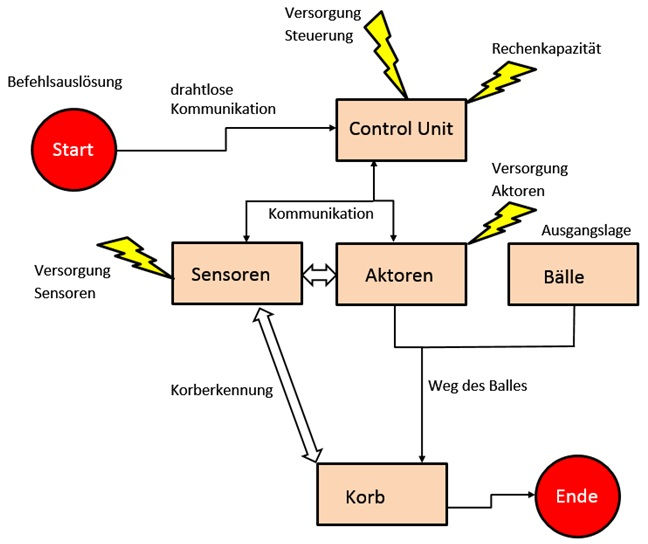
\includegraphics[width=0.9\textwidth]{Morphologie/Bilder/Blockschaltbild.jpg}
		\centering
		\caption{Funktionsskizze zur Aufgabenstellung}
		\label{abb:Blockschaltbild} 
	\end{figure}
	
	Aus der Abbildung \ref{abb:Blockschaltbild} ergeben sich folgende Teilprobleme:
	\begin{itemize}
		\item Startgerät / Endgerät
		\item Startbefehlsübermittlung (drahtlos)
		\item Rechenkapazität (immer inklusive Verteileinheit)
		\item Versorgung der Steuerung / Sensoren
		\item Sensorik (Korberkennung)
		\item Ausgangslage der Bälle
		\item Weg des Balles (zum Korb)
	\end{itemize}
	Als nächster Schritt werden die Teilprobleme genauer definiert. Der Technologierecherche entspringende Lösungsansätze sollen die Problembereiche möglichst gut abdecken.
	
	\subsection{Beurteilung der Teilprobleme}
		Durch die Definition von passenden Beurteilungskriterien sollen die verschiedenen Lösungsansätze für ein Teilproblem taxiert werden. An dieser Stelle bieten sich die definierten Ziele der Teamcharta an:
		
		\begin{enumerate}
			\item Treffgenauigkeit
			\item Geschwindigkeit
			\item Gewicht
		\end{enumerate}
		Der Faktor Zuverlässigkeit erhält in jedem Teilproblem eine hohe Wert, dies aufgrund der Zielsetzung die eine hohen Zuverlässigkeit aller beteiligten Elemente nach sich zieht. Der Aufwand belegt in der Regel einen kleinen Faktor, da er in einem Schulprojekt einen sekundären Stellenwert hat. Der Faktor der Kosten wurde bewusst im Mittelfeld angesiedelt, um den Fokus auf die Zielsetzung zu legen, aber trotzdem teuren Produkten ein Nachteil einzuhandeln.
		In der Regel ist die Verteilung der Punkte pro Kriterium so geregelt, dass die schlechteste Lösung 1 Punkt erhält, die beste Lösung 5 Punkte, der Rest einen Wert dazwischen.\\
		\\
		Um die nachfolgenden Beschreibung zu den Kriterien richtig zu interpretieren, ist die Beurteilung in Anhang \ref{apx:Beurteilung} zusätzlich zum jeweiligen beschreibenden Text hinzuzuziehen. 
		\begin{itemize}
			\item Ausgangslage der Bälle (Annahme: Kugel (gefüllt mit Bällen) muss geometrisch sein)
				\begin{itemize}
					\item Geschwindigkeit\\
					Alle Bälle in einer grossen Kugel braucht wenig Zeit, ist daher die beste Lösung. Der Drehkranz ist schwerfällig und langsam.
					\item Gewicht\\
					Der Trichter ist eine einfache, minimalistische Konstruktion, die wenig Gewicht aufweist. Der Drehkranz ist eine grosse, schwere Konstruktion mit mehreren Aktoren.
					\item Zuverlässigkeit\\
					Die Bälle in einem Trichter können schnell verstopfen. Ein sauber konstruiertes und aufgebautes Magazin ist sehr zuverlässig. 
					\item Kosten\\
					Der Trichter hat eine einfache, minimalistische Konstruktion, benötigt daher wenig Material. Der Drehkranz hat viele Aktoren und ein aufwändiges Design.
					\item Aufwand\\
					Die Umsetzung eines Trichters ist einfach und schnell erledigt. Der Drehkranz ist aufwändig.					
				\end{itemize}
			\item Rechenkapazität (Annahme: Embedded Prozessor günstiger Bauart)
				\begin{itemize}
					\item Zuverlässigkeit\\
					Smartphone und Embedded Prozessoren sind sehr zuverlässig, da sie on-board sind. Ein Notebook als Recheneinheit ist aufgrund der vielen Datenübermittlung fehleranfällig.
					\item Geschwindigkeit\\
					Embedded Prozessoren sind für genau eine spezifische Aufgabe ausgelegt und dimensioniert. Ein Notebook als Recheneinheit ist aufgrund der vielen Datenübermittlung fehleranfällig und langsam.
				 	\item Gewicht\\
				 	Embedded Prozessoren sind für genau eine spezifische Aufgabe ausgelegt und dimensioniert, beinhalten nur das absolut Nötigste. Das Smartphone wird als Teil des Produktegewichts gerechnet.
					\item Kosten\\
					Das Smartphone/Notebook wird von einem Teammitglied zur Verfügung gestellt. Ein eingebetteter Prozessor müsste zugekauft werden.
					\item Aufwand\\
					Für einen Embedded Prozessor müsste eine eigene Stromversorgung, drahtlos-Kommunikations-Modul, etc. gebaut werden. Ein Notebook beruht auf wohlbekannten, gut dokumentierten Technologien.
				\end{itemize}
				
			\item Sensorik
				\begin{itemize}
					\item Geschwindigkeit\\
					Eine Foto mit einer Smartphone Kamera ist schnell geschossen und kann direkt im Smartphone bearbeitet werden. Ein Laser muss viele Punkte abscannen und dabei mechanisch geschwenkt werden.
					\item Genauigkeit\\
					Ein Laser misst viele Punkte, kann daher ein sehr detailliertes Abbild schaffen. Ultraschallmessungen sind laut Recherchen nicht sehr präzise.  
					\item Zuverlässigkeit\\
					Laservermessungen sind dank des detaillierten Abbilds sehr zuverlässig in der Korberkennung. Infrarot ist aufgrund des vielen Fremdeinflusses (bsp. Lichtstrahler an Spielfeldrand) sehr unzuverlässig.
					\item Kosten\\
					Das Smartphone mit integrierter Kamera wird von einem Teammitglied zur Verfügung gestellt. Für einen Laser muss aufgrund der mechanischen Justierung zusätzliche Bauteile eingekauft werden.
					\item Aufwand\\
					Ein Smartphone mit integrierter Kamera beruht auf wohlbekannten, gut dokumentierten Technologien. Für einen Laser muss aufgrund der mechanischen Justierung zusätzlichen Aufwand betrieben werden
				\end{itemize}
				
			\item Startbefehlsübermittlung
				\begin{itemize}
					\item Zuverlässigkeit\\
					Bluetooth (und WLAN) basieren auf wohlbekannten, gut dokumentierten, standardisierten Technologien. Akustische Signale können einfach generiert und damit den Prozess erheblich stören.
					\item Kosten\\
					Bluetooth (und WLAN) sind Teil der eingebauten Technologie in einem modernen Smartphone / Notebook. Bei Infrarot und Akustischen Signalen kostet der Empfänger.
					\item Aufwand\\
					Bluetooth (und WLAN) sind Teil der eingebauten Technologie in einem modernen Smartphone / Notebook und beruhen auf wohlbekannten, gut dokumentierten, standardisierten Technologien. Das Auswerten eines Akustischen Signals ist aufwändig, fehleranfällig und benötigt zusätzliche Elektronik.
				\end{itemize}
				
			\item Startgerät – Endgerät
				\begin{itemize}
					\item Zuverlässigkeit\\
					Ein Notebook beruht auf wohlbekannten, gut dokumentierten, erprobten Technologien (drahtlos Kommunikation, sowie dazugehöriger Software). Taster muss neu gebaut werden, kann daher fehleranfällig sein.
					\item Kosten\\
					Das Smartphone/Notebook wird von einem Teammitglied zur Verfügung gestellt. Ein Taster müsste neu gebaut respektive eingekauft werden.
					\item Kompatibilität\\
					Ein Smartphone besitzt nur ein Betriebssystem mit beschränkten Funktionen. Mit einem Notebook kann man viele verschiedene Software-Lösungen erstellen.
					\item Aufwand\\
					Das Smartphone/Notebook wird von einem Teammitglied zur Verfügung gestellt, es entsteht vor allem softwaretechnischer Aufwand. Für einen Taster müsste ein eigenes kleines System entwickelt werden.
				\end{itemize}
				
			\item Versorgung Steuerung / Sensorik
				\begin{itemize}
					\item Zuverlässigkeit\\
					Ein Akku hat im Vergleich zu einem Netzteil höhere Spannungsschwankungen.
					\item Gewicht\\
					(hier als Vorteil, da als Ballast anrechenbar) Akku kann zur Gewichtsbestimmung entfernt werden.
					\item Kosten\\
					Netzteile sind günstig und alte Netzteile können für diese Aufgabe recycelt werden. Akkus müssten neu gekauft werden.
					\item Aufwand\\
					Netzteile können in kompletter Form gekauft werden. Akku’s müssen mit Elektronik stabilisiert und geregelt werden.
				\end{itemize}
				
			\item Weg des Balles (Nachfolgende Bezeichnungen (..) beziehen sich auf die Nummerierung im Anhang \ref{apx:Beurteilung})			
				\begin{itemize}
					\item Geschwindigkeit\\
					Je weniger Achsen bewegt werden müssen, desto schneller ist die jeweilige Lösung. (2) muss nur eine Drehbewegung ausführen. (5) muss drei Bewegungen ausführen.
					\item Zuverlässigkeit\\
					Je weniger Achsen bewegt werden müssen, desto zuverlässiger ist die Lösung. (2) muss nur eine Drehbewegung ausführen. (1) muss fliegen und zusätzlich noch ständig nachkorrigieren, äussre Störeinflüsse schwer vorauszusagen.
					\item Genauigkeit\\
					Je mehr Achsen bewegt werden müssen, je mehr Toleranzen, Fehler und Justierungen treten ein. (2) hat nur eine bewegliche Achse. (1) und (5) haben viele bewegliche Achsen und viele unbekannte Störeinflüsse.
					\item Gewicht\\
					Je mehr Achsen bewegt werden müssen, je mehr Antriebe, Materialien und Elektronik wird benötigt. (2) ist stationär. (4) und (5) haben viele bewegliche Achsen. 
					\item Kosten\\
					Je mehr Achsen bewegt werden müssen, je teurerer werden die jeweiligen Ausführungen. (2) ist stationär. (4) und (5) haben viele bewegliche Achsen. (1) kann zudem im Testfall abstürzen und so teure Teile zerstören.
					\item Aufwand\\
					(1) softwaretechnischer Aufwand ist immens. (2) stationäre Lösung im Vergleich eher einfach zu realisieren. (4) und (5) haben viele bewegliche Achsen, jede zusätzliche Achse erfordert weiteren Aufwand.	
				\end{itemize}
		\end{itemize}


  	 \begin{landscape}
	\section{Grobkonzept}
		\begin{figure}[h!]
			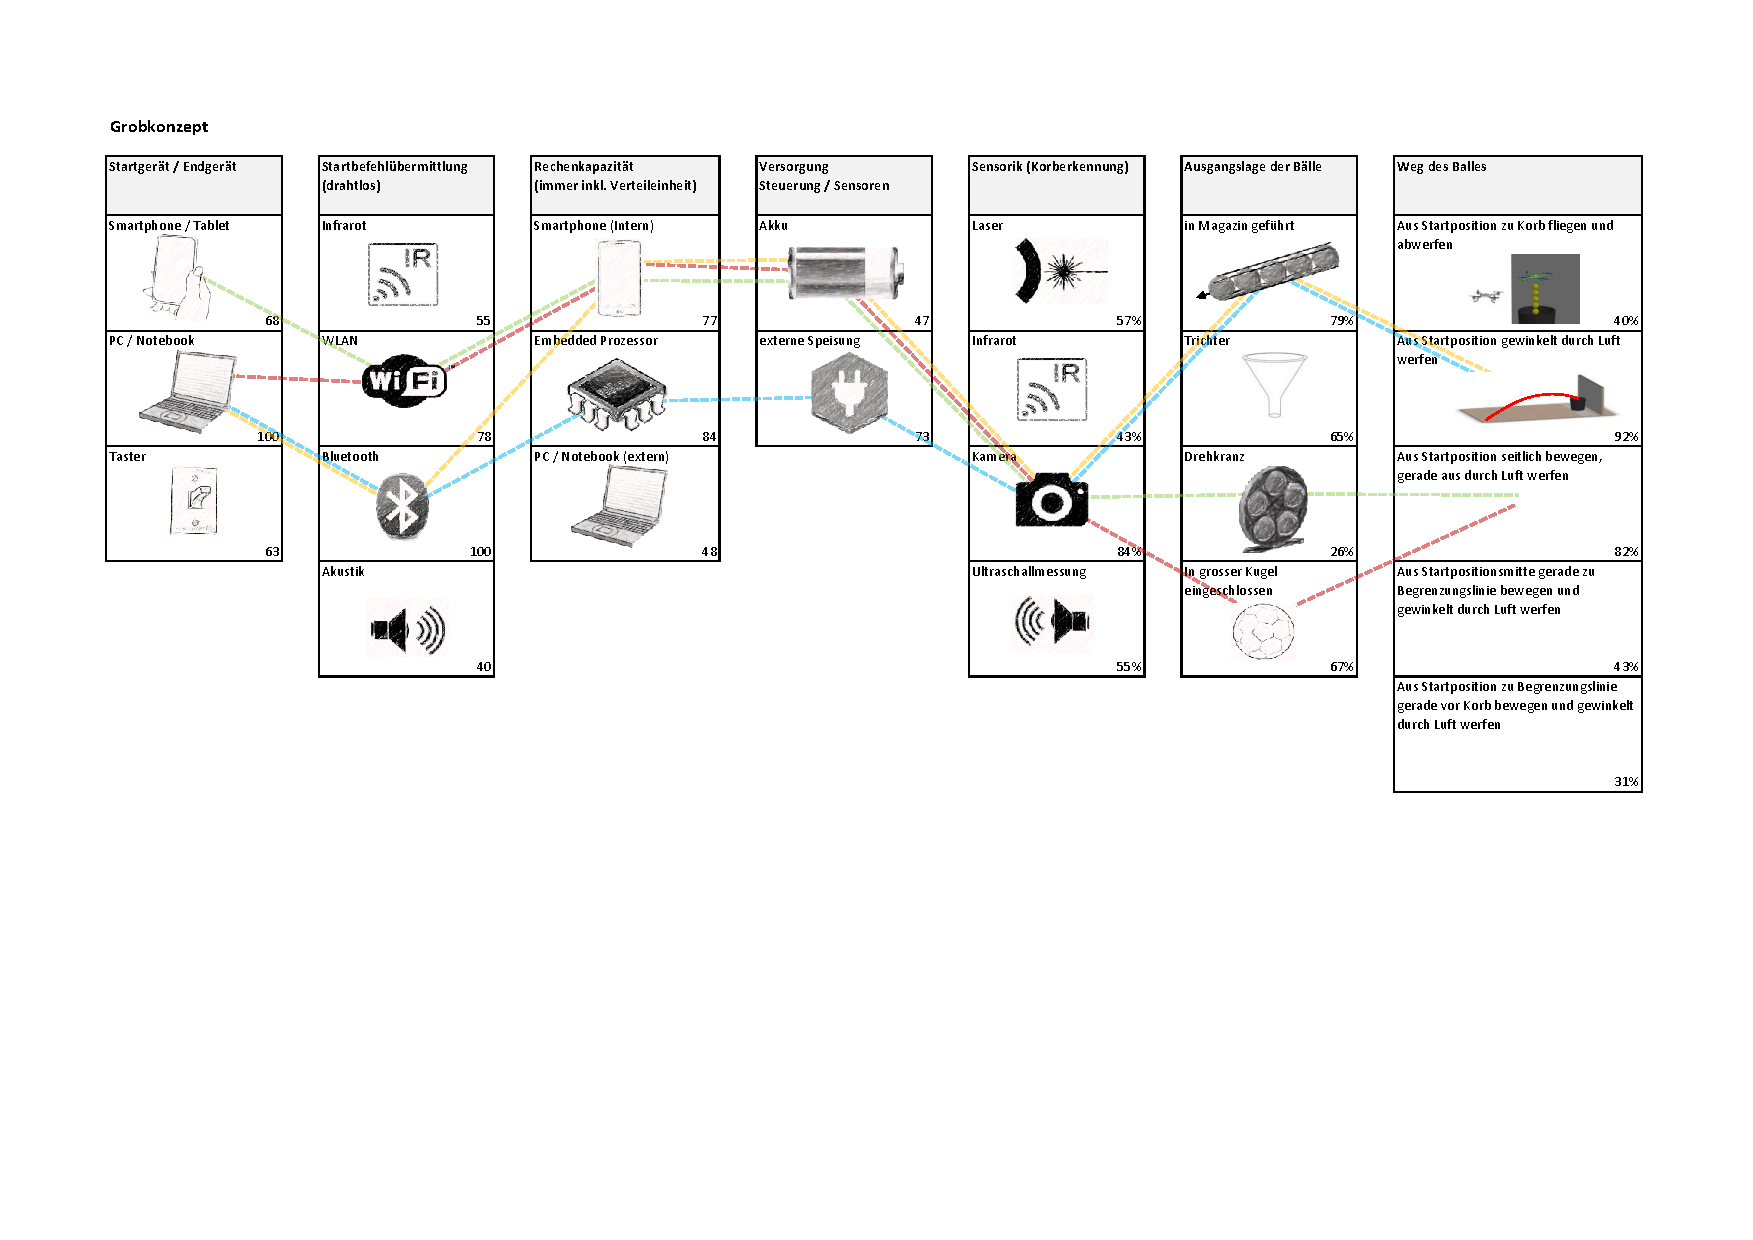
\includegraphics[page=1,scale=0.75,clip,trim=17mm 37mm 21mm 19mm]{Morphologie/Bilder/Grobkonzept.pdf}
			\centering
			\caption{Grobkonzept} 
			\label{abb:Grobkonzept}
		\end{figure}	
\end{landscape} 

\parindent0pt{\textit{Die detaillierte Bewertung aller Varianten sind dem Anhang \ref{apx:BewertungGrobkonzepte} zu entnehmen.}}\\
\\
Es wurden vier Varianten (orange, grün, rot, blau), wie in Abbildung \ref{abb:Grobkonzept} ersichtlich, gewählt. 
\begin{itemize}
	\item Blaue Variante\\
	Eine Auswahl aller Lösungen, welche die höchste Punktezahl durch die Bewertungskriterien erreichte.
	
	\item Rote Variante\\
	Ausgangspunkt in dieser Variante ist die Auswahl, die Bälle in eine Kugel einzuschliessen. Da ein Smartphone mit integrierter Kamera verwendet wird, kann man zwei Teilprobleme mit einem Gerät lösen. Den Weg des Balles via seitliche Verschiebung wurde aufgrund der Unhandlichkeit der grossen Kugel gewählt: der Weg soll kurz und einfach gehalten werden. Der Akku dient in dieser Variante neben der Energieversorgung auch als Ballast, um dem grossen Gewicht der Kugel entgegenzuwirken. Weiter ist die Ausgabe des Startsignals mit einem Notebook, sowie die Übertragung mit WLAN leicht zu Realisieren, da diese Lösungen auf gut dokumentierten Technologien basieren.
	
	\item Grüne Variante\\
	Für die grüne Variante wurde als Ausgangslage der Bälle die Führung in einem Drehkranz gewählt. Kongruent zur Variante Rot, wurde auch hier der Weg des Balles via seitliche Verschiebung aufgrund der Unhandlichkeit des Drehkranzes als Favorit erkoren. Für die Wahl des Akkus, der Startsignal-Übertragung per WLAN und die Verwendung eines Smartphones überzeugten dieselben Kriterien, welche bereits in der roten Variante genannt wurden.
	
	\item Orange Variante\\
	Aus der Startposition gewinkelt werfen, ist der Ursprung der orangen Variante. Eine geführte Ausgabe aus einem Magazin hat den Vorteil, dass es mit leichten Materialen gebaut werden kann, verschiedene Formen, Winkel und Ausgabegeschwindigkeiten zur Verfügung stehen. Der Akku dient in dieser Variante neben der Energieversorgung auch als Ballast und hat den schönen Nebeneffekt, dass das System energieautark ist.
\end{itemize}

\subsection{Entscheidung}
Die orange Variante bietet als gesamtes Konzept die erfolgversprechendste und effizienteste Lösung, bezüglich der vordefinierten Ziele der Team-Charta. Den Ball von der Startposition aus gewinkelt durch die Luft zu werfen erfordert keine zusätzlichen Bauteile um das Produkt am Boden zu verschieben. Dies minimiert einerseits den Aufwand und verringert die Fehleranfälligkeit erheblich. Die Bälle in der Ausgangslage in einem Magazin zu führen hat den Vorteil, dass eine allfällige stückweise Ausgabe der Bälle mit wenig Aufwand hinzugefügt werden kann. Ein Smartphone mit integrierter Kamera löst die zwei Teilprobleme der Korberkennung und Rechenkapazität mit einem Gerät. Des weiteren wäre das Produkt durch die Verwedung eines Akkus energieautark. Die Ausgabe des Startsignals und Endsignals mit einem Notebook und die Übermittlung mit Bluetooth sind einfach auszuführen und beruhen auf wohlbekannten, gut dokumentierten Technologien.
  	 \newpage
  	 \parindent0pt{\Large{\textcolor{red}{Dieses Kapitel ist noch nicht offiziell Bestandteil des Testat 2.}}}
\section{Feinkonzept}
	Nach der Entscheidung für ein Grobkonzept folgt nun die Detaillierung dieses Konzeptes in ein Feinkonzept. Die ursprünglich sieben Teilprobleme wurden in 19 Subteilprobleme auf gesplittet. Zu all diesen Subteilproblemen existieren wiederum Lösungsvarianten, die in Abbildung \ref{abb:Feinkonzept} dargestellt sind.
	
	\begin{figure}[h!]
		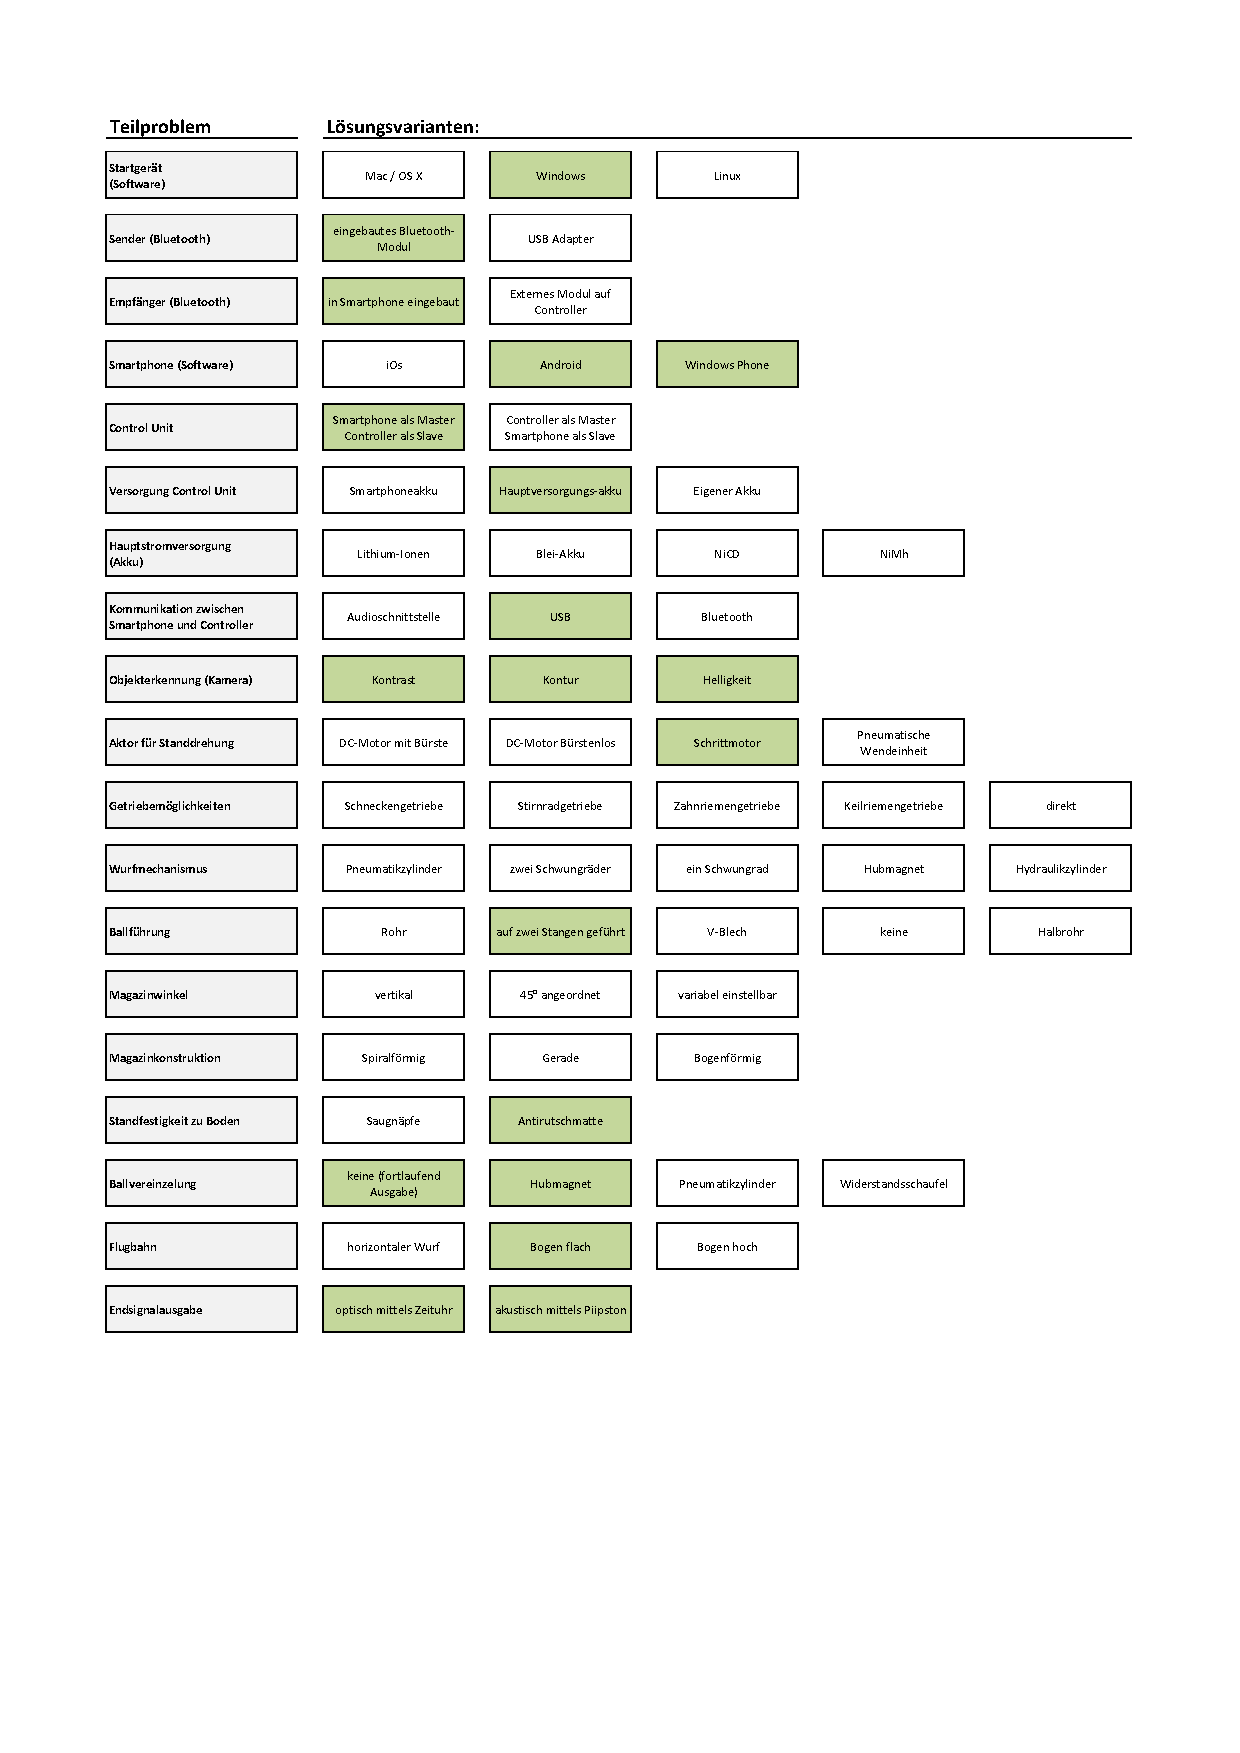
\includegraphics[page=1,scale=0.77,clip,trim=17mm 70mm 18mm 20mm]{Morphologie/Bilder/Feinkonzept.pdf}
		\centering
		\caption{Feinkonzept}
		\label{abb:Feinkonzept} 
	\end{figure}
	
	Die grün eingefärbten Lösungsvarianten in Abbildung \ref{abb:Feinkonzept} stellen unsere Entscheidung im jeweiligen Subteilproblem dar. Nachfolgend ist eine Erklärung zur Lösungsfindung zu jedem einzelnen Subteilproblem beschrieben.\\
	\\	
	\textbf{Startgerät (Software})\\
	Als Startgerät wird ein Notebook mit dem Windows-Betriebssystem verwendet, da es ein viel verbreitetes, stabiles, gut dokumentiertes Betriebssystem ist und alle nötigen Funktionen zur Ausführung unserer Problemstellung hat. Keines der Teammitglieder verwendet ein Notebook mit Mac/OSX oder Linux, diese beiden Betriebssysteme kommen daher nicht in Frage.\\
	\\
	\textbf{Sender (Bluetooth)}\\
	Das eingesetzte Notebook hat ein eingebautes Bluetooth-Modul welches als Sender verwendet werden kann, daher wird ein USB-Bluetooth-Adapter überflüssig.\\
	\\
	\textbf{Empfänger (Bluetooth)}\\
	Als Empfänger auf der Seite des Ballwerfers wird das im Smartphone integrierte Bluetooth-Modul verwendet. Das Smartphone agiert in diesem System als Master, der Controller übernimmt die Rolle des Slaves.\\
	\\
	\textbf{Smartphone (Software)}\\
	Beim Smartphone-Betriebssystem kommen nur die Open source Variante Android und das Windows-Phone-Betriebssystem in Frage, da sie bezüglich Zugriff auf die vorhandenen Schnittstellen nicht eingeschränkt sind. Eine genaue Festlegung ist zurzeit noch nicht möglich. Definitiv ausgeschlossen ist das iOS Betriebssystem von Apple, da keine Programmiererfahrung auf diesem Gebiet vorhanden ist und der Zugriff auf die nötigen Schnittstellen eingeschränkt ist.\\
	\\
	\textbf{Versorgung Control-Unit}\\
	Der Hauptversorgungsakkumulator soll die Versorgung der Control-Unit übernehmen.\\
	\\
	\textbf{Hauptstromversorgung (Akkumulator)}\\
	Die Art des Hauptversorgungsakkumulators wird erst mit der Konstruktion und Dimension des Produkts klar, bleibt im daher im Moment noch offen.\\
	\\
	\textbf{Kommunikation zwischen Smartphone und Controller}\\
	Die Kommunikation des Smartphones zum Controller findet via USB-Kabel statt. Dies Aufgrund der Controller-Wahl, der nur die Kommunikation mit USB zulässt.\\
	\\
	\textbf{Objekterkennung (Kamera)}\\
	Bei der Objekterkennung mittels Kamera werden idealerweise alle drei optischen Bestimmungskriterien Kontrast, Helligkeit und Kontur zur Objektidentifikation verwendet. Falls die Erkennung mittels Kamera nicht realisierbar ist, stellt Ortung via Ultraschall eine interessante Alternative dar.\\
	\\
	\textbf{Aktor für Standdrehung}\\
	Die Drehung der Plattform erfolgt direkt durch einen Schrittmotor, da diese Lösung kleine Veränderungen des Winkels zulässt und in gleichmässigen Schritten gesteuert werden kann.\\
	\\
	\textbf{Getriebemöglichkeiten}\\
	Ob Getriebemöglichkeiten zum Einsatz kommen, ist durch den momentanen Stand des Produkts nicht gegeben.\\
	\\
	\textbf{Wurfmechanismus}\\
	Der Pneumatikzylinder erlaubt eine hohe Wurfreproduzierbarkeit. Mithilfe zweier Schwungräder kann durch einbringen eines Dralls die Flugbahn stabilisiert werden. Bei nur einem Schwungrad besteht der Vorteil, dass nur ein Motor verwendet werden muss. Ein Hubmagnet bietet eine gute Alternative zur Pneumatik-Ausführung, da keine externe Druckluft-Versorgung nötig ist. Der Hydraulikzylinder fällt aufgrund der niedrigen Geschwindigkeit weg. Die genaue Auswahl des Wurfmechanismus wird durch die Testbauten ermittelt.\\
	\\
	\textbf{Ballführung}\\
	Die Ausführung auf zwei oder mehr Stangen ist bauleicht und hat wenig Laufwiederstand für den Ball. In einem geschlossenen und halboffenen Rohr ist die Gefahr von Verstopfungen und Laufreibungen der Bälle höher als bei einer Lösung mittels Stangen.\\
	\\
	\textbf{Magazinwinkel und Magazinkonstruktion}\\
	Der Magazinwinkel und Magazinkonstruktion kann erst im Zusammenhang mit der Gesamtlösung respektive des Wurfmechanismus erarbeitet werden.\\
	\\
	\textbf{Standfestigkeit zu Boden}\\
	Die Standfestigkeit soll mittels Antirutschmatte gewährleistet werden, falls dies nicht genügt, können Saugnäpfe verwendet werden.\\
	\\
	\textbf{Ballvereinzelung}\\
	Falls es die Umstände zulassen, wird auf eine Ballvereinzelung verzichtet, wenn sie aber aufgrund des Wurfmechanismus nötig wird, soll ein Hubmagnet als Schieber zum Einsatz kommen.\\
	\\
	\textbf{Flugbahn}\\
	Die Flugbahn soll in einem flachen Bogen erfolgen, um das Gerät mit einen möglichst tiefen Schwerpunkt auszustatten und dass der Ball nicht aus dem Korb zurückspringen kann.\\
	\\
	\textbf{Endsignalausgabe}\\
	Die akustische und optische Endsignalausgabe erfolgt laut Aufgabenstellung auf dem Startgerät (Notebook).\\

  	 
  	 %  Detaillierte Berechnungen 
  	 
  	 %  Versuche und Tests: Details, Messprotokolle etc.
  	 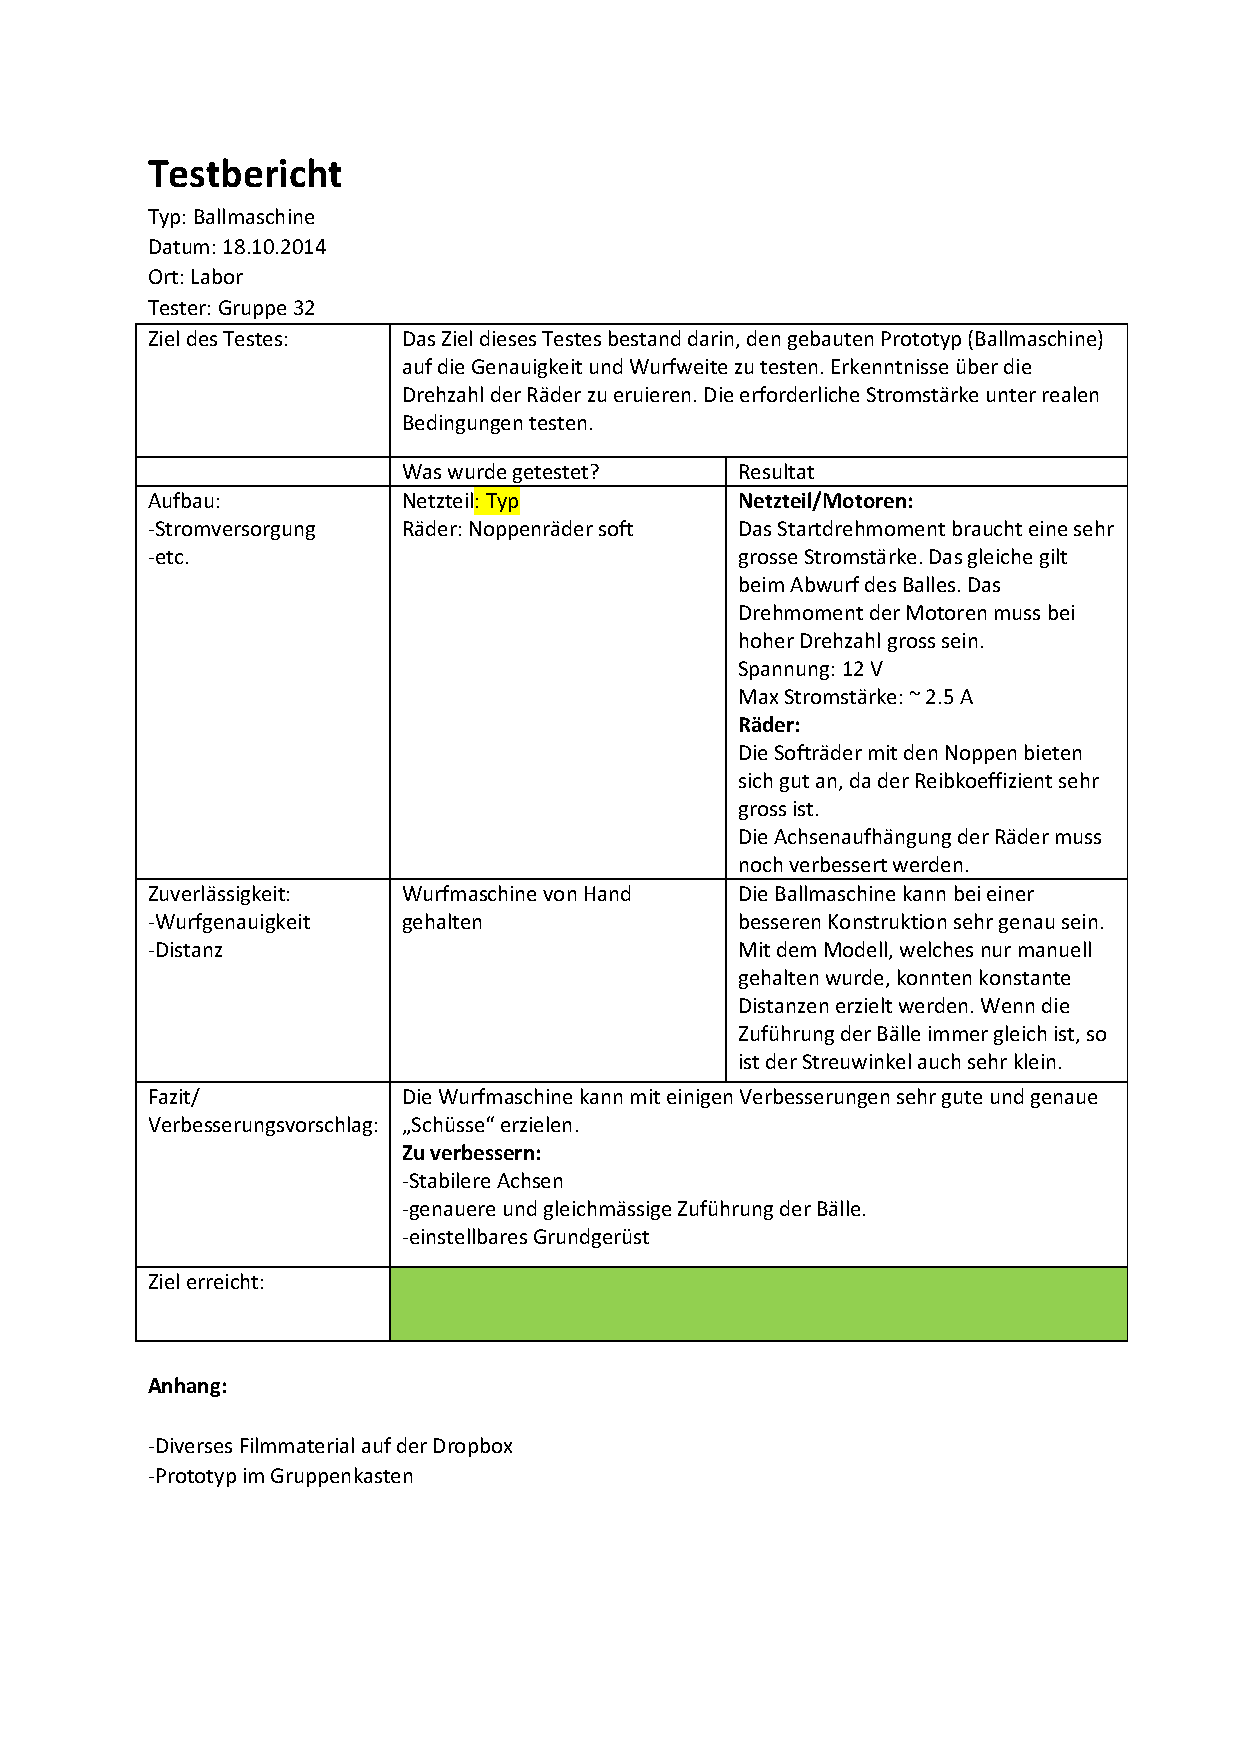
\includegraphics[page=1,width=1\textwidth]{Funktionstests/Ballmaschine.pdf}
  	 \newpage
  	 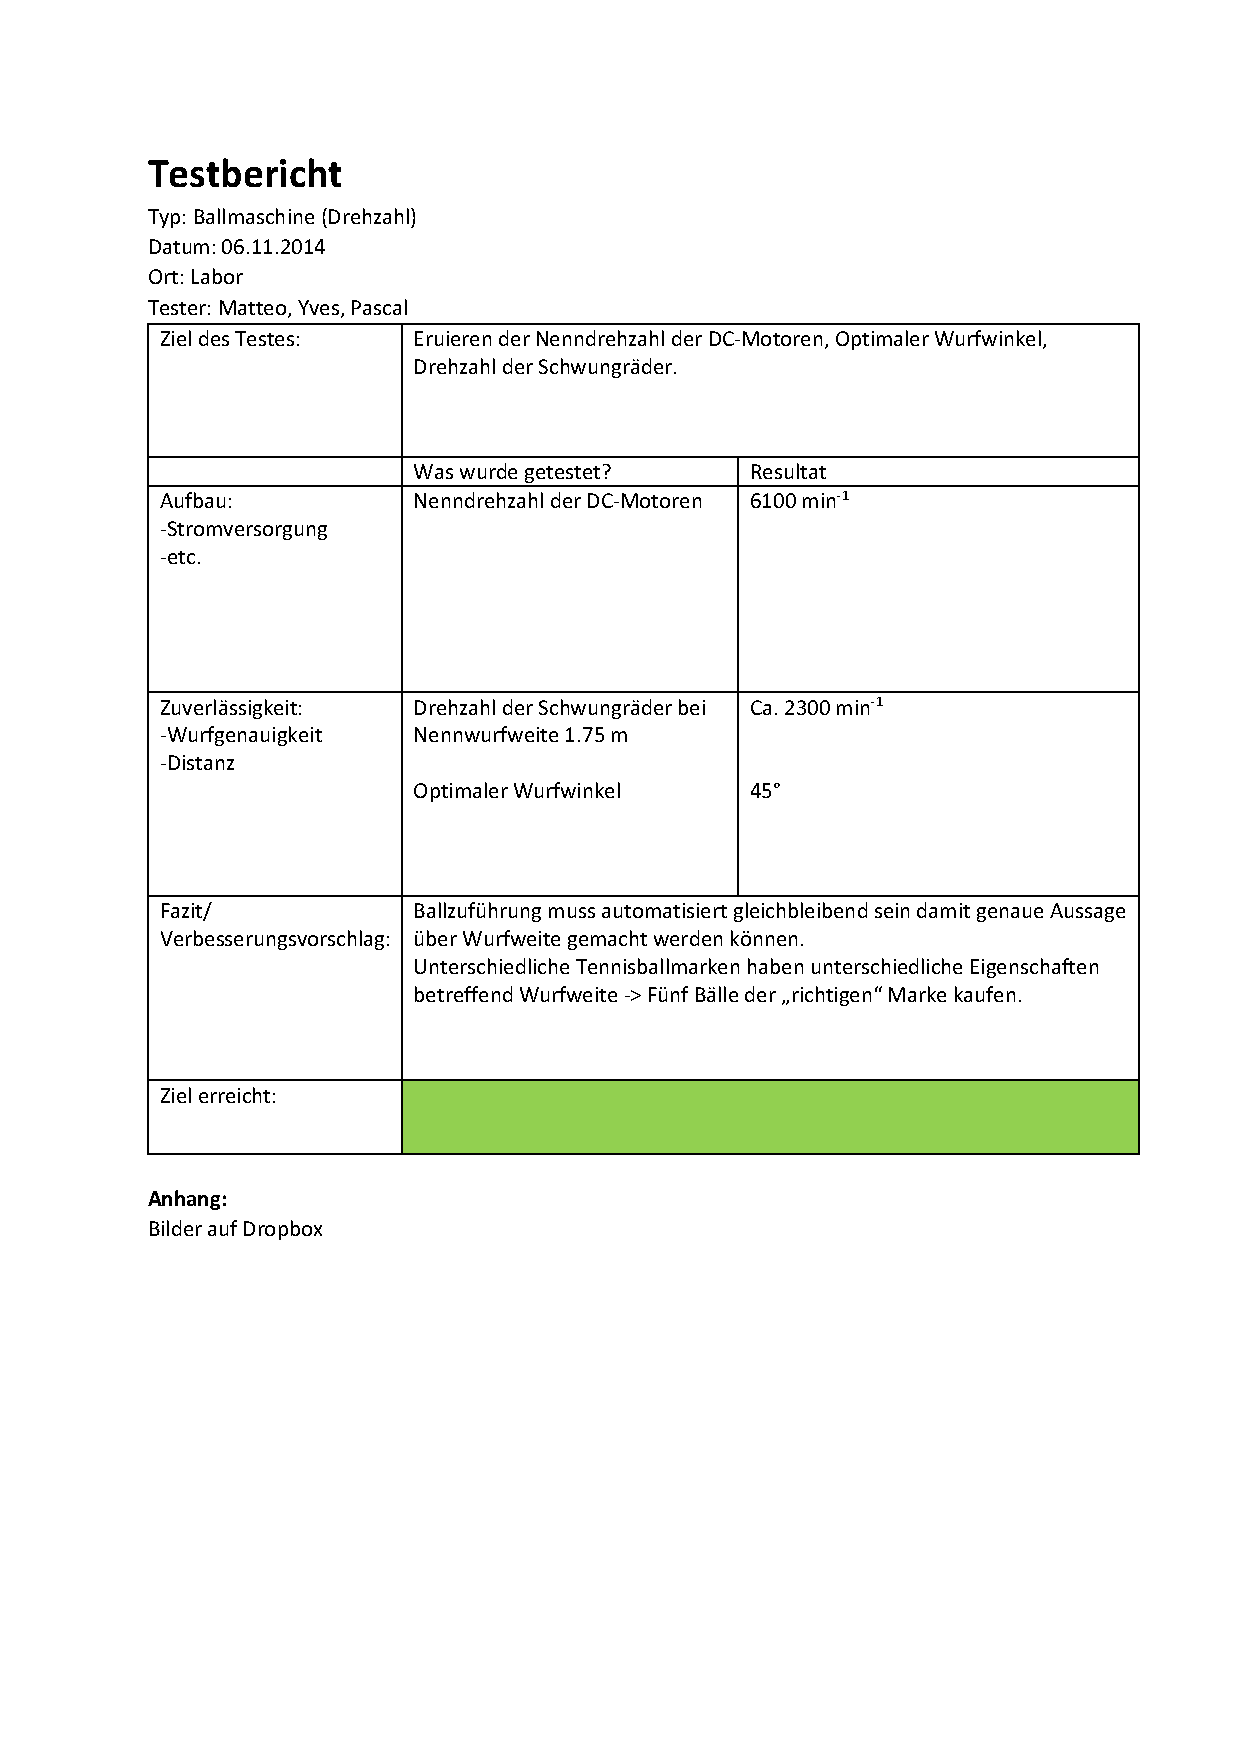
\includegraphics[page=1,width=1\textwidth]{Funktionstests/BallmaschineDrehzahl.pdf}
  	 \newpage
  	 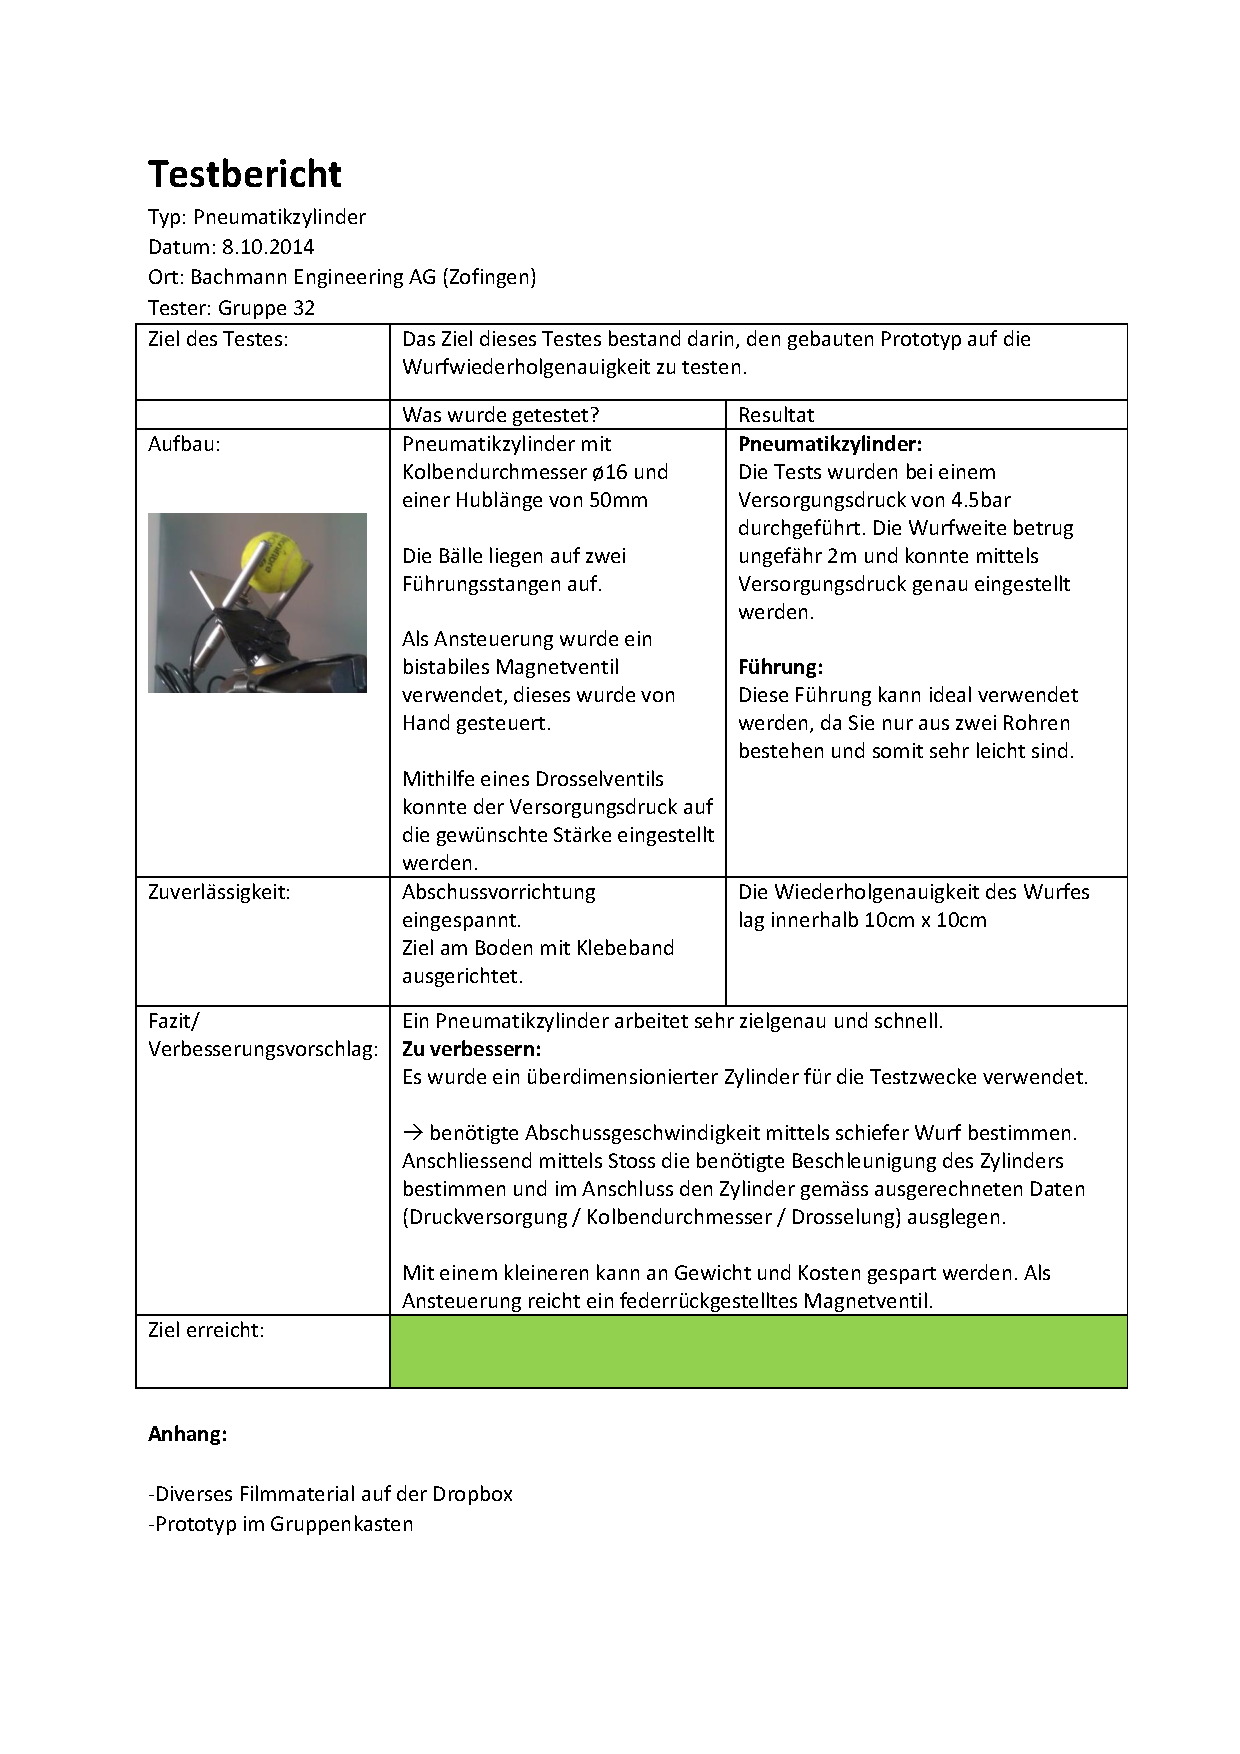
\includegraphics[page=1,width=1\textwidth]{Funktionstests/Pneumatikzylinder.pdf}
  	 \newpage
  	 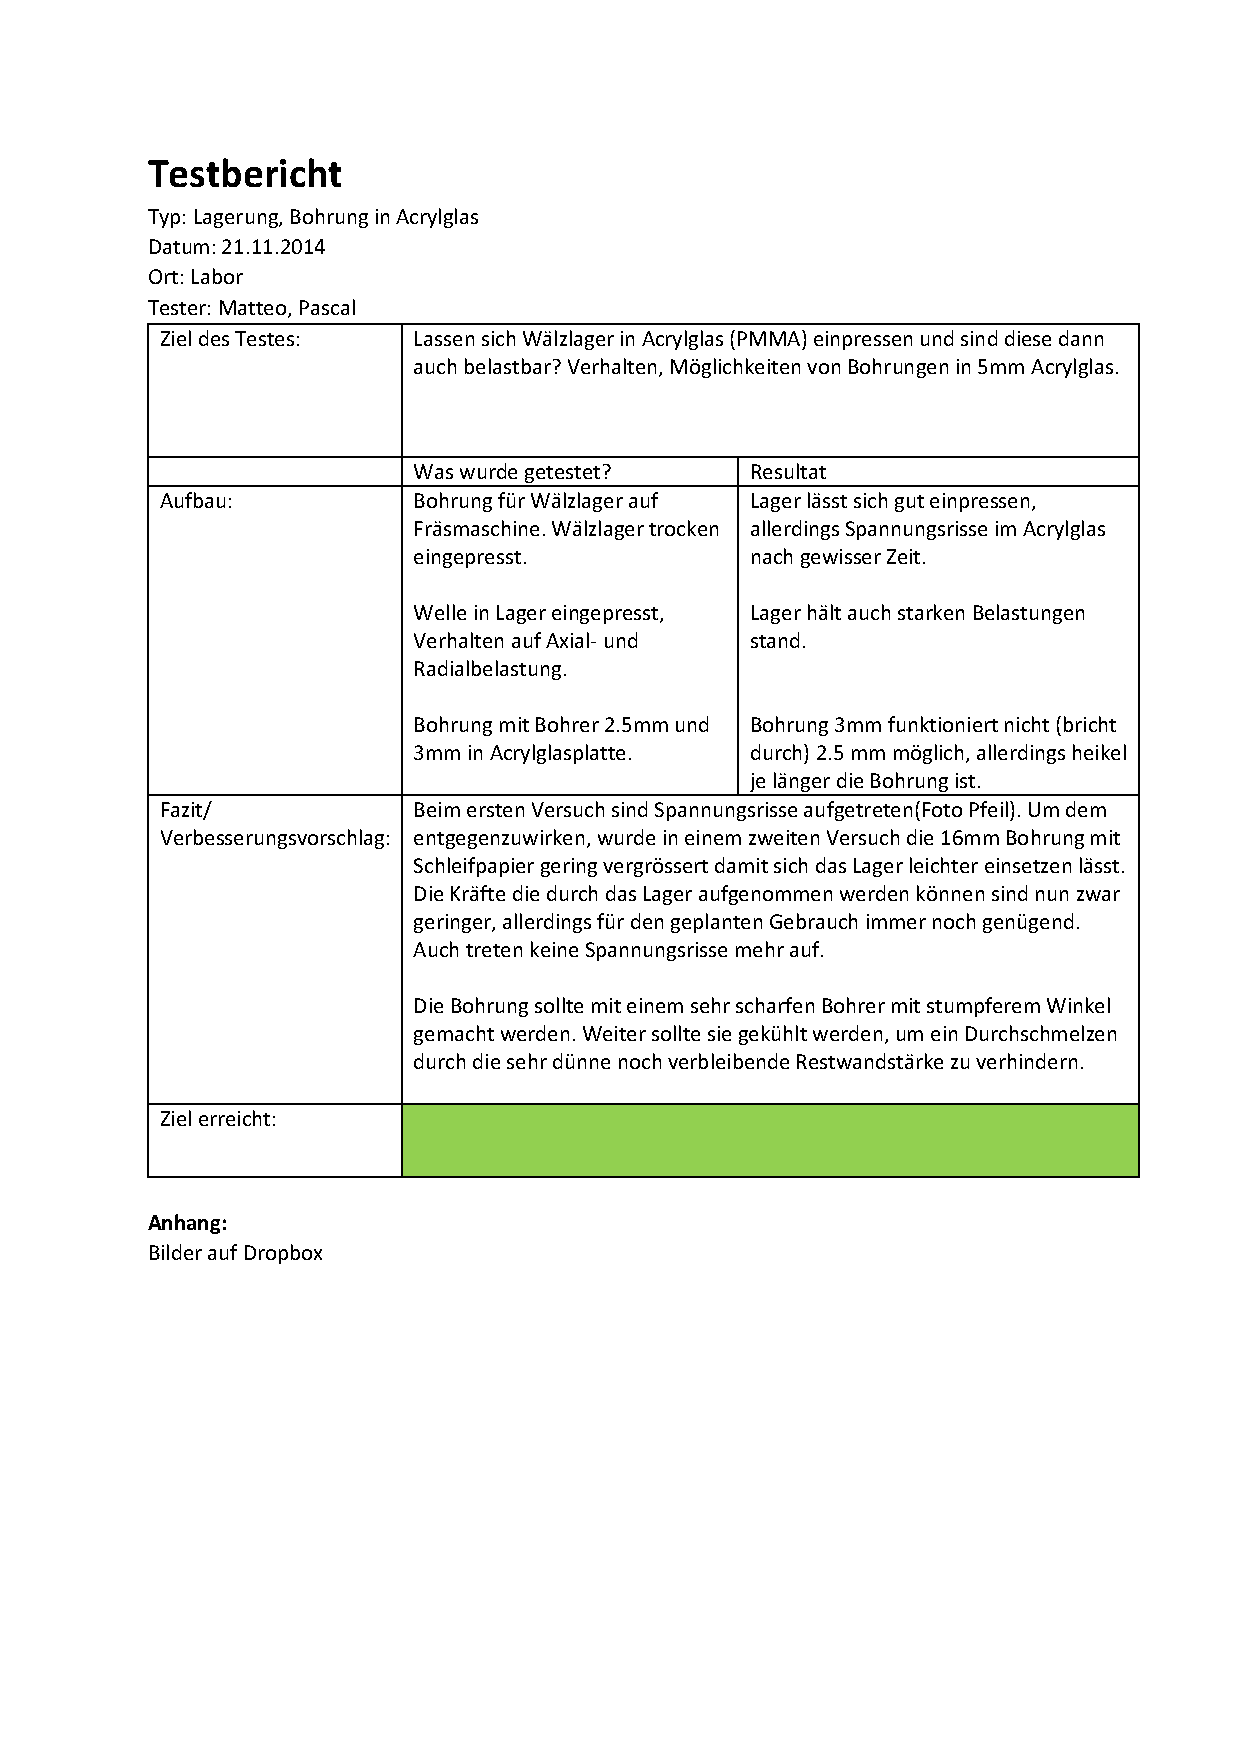
\includegraphics[page=1,width=1\textwidth]{Funktionstests/Acrylglas.pdf}
  	 \newpage
  	 
  	 
  	 %  Meilensteinberichte, Protokolle, Pendenzenlisten
  	 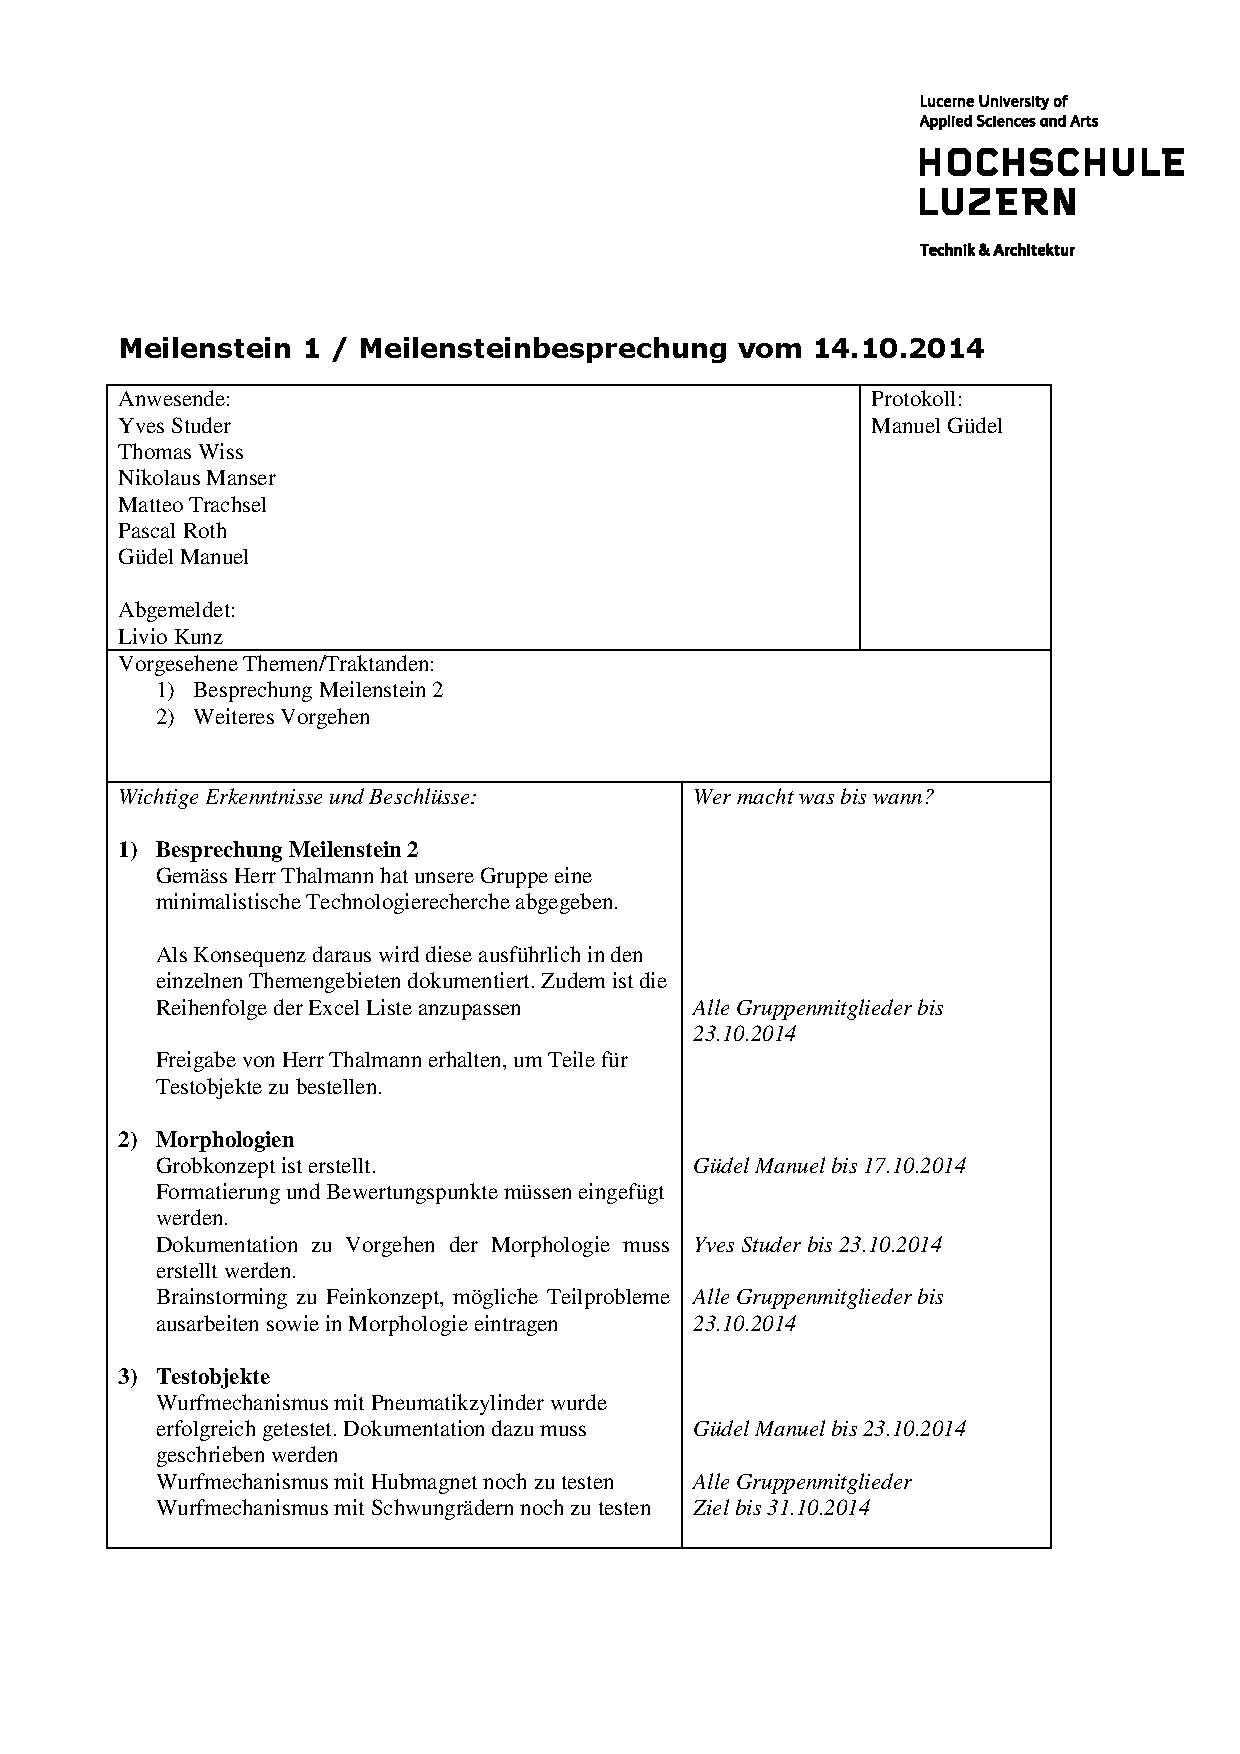
\includegraphics[page=1,width=1\textwidth]{Anhangsdokument/Besprechung_MS1.pdf}
  	 \newpage
  	 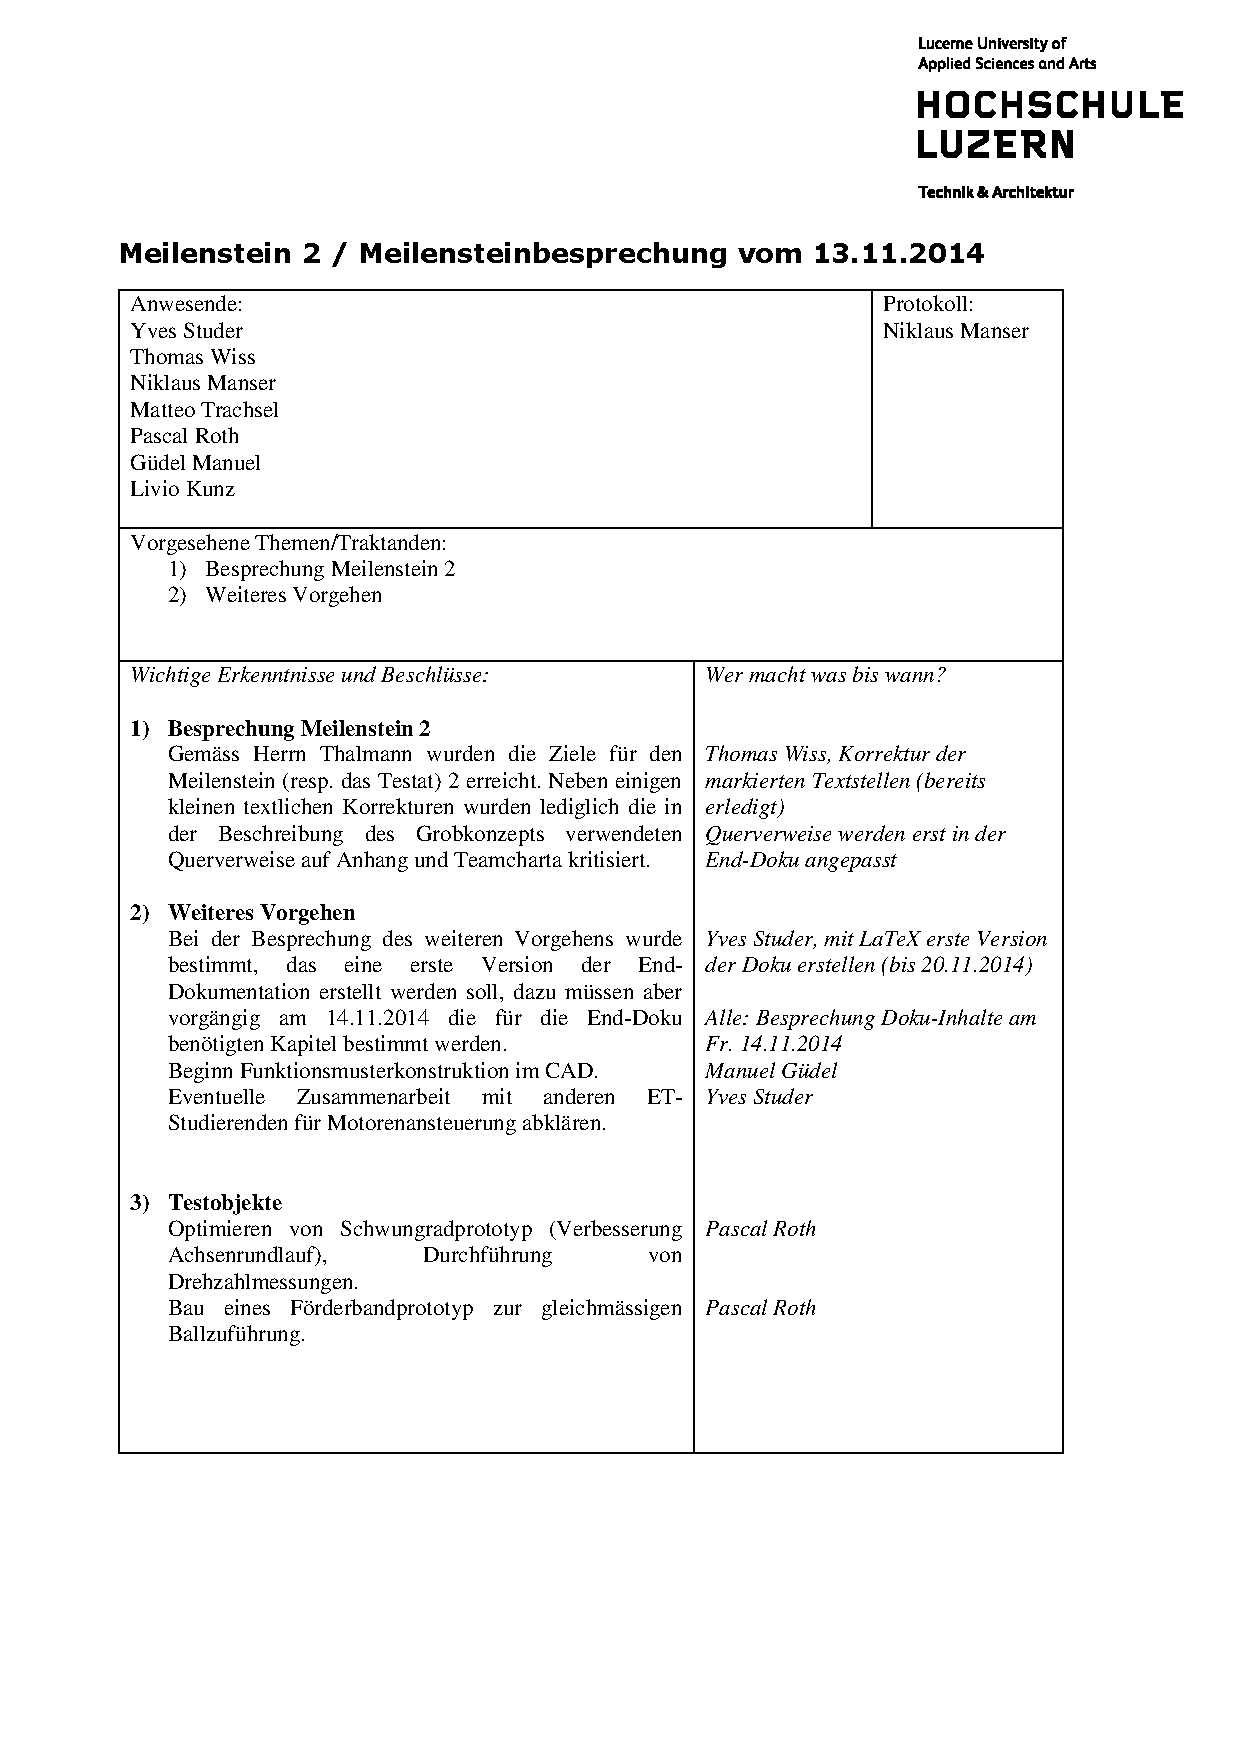
\includegraphics[page=1,width=1\textwidth]{Anhangsdokument/Besprechung_MS2.pdf}


    
    \newpage
    \listoffigures      
    
    \begin{flushleft}
        \renewcommand{\refname}{Literatur- und Quellenverzeichnis}
    \end{flushleft}
    \appendix
    % Beginn des Anhangs
        \begin{appendix}
            \clearpage
            \pagenumbering{Roman} % römische Nummerierung des Anhangs (Grosse Buchstaben)
            %\section{Anhang}
            %\newpage
            \section{Anhang}
            \begin{landscape}
	\section{Beurteilung der Teilprobleme}
	\label{apx:BeurteilungTeilprobleme}
		\subsection{Ausgangslage der Bälle}
		\label{apx:AusgangslageDerBaelle}}
		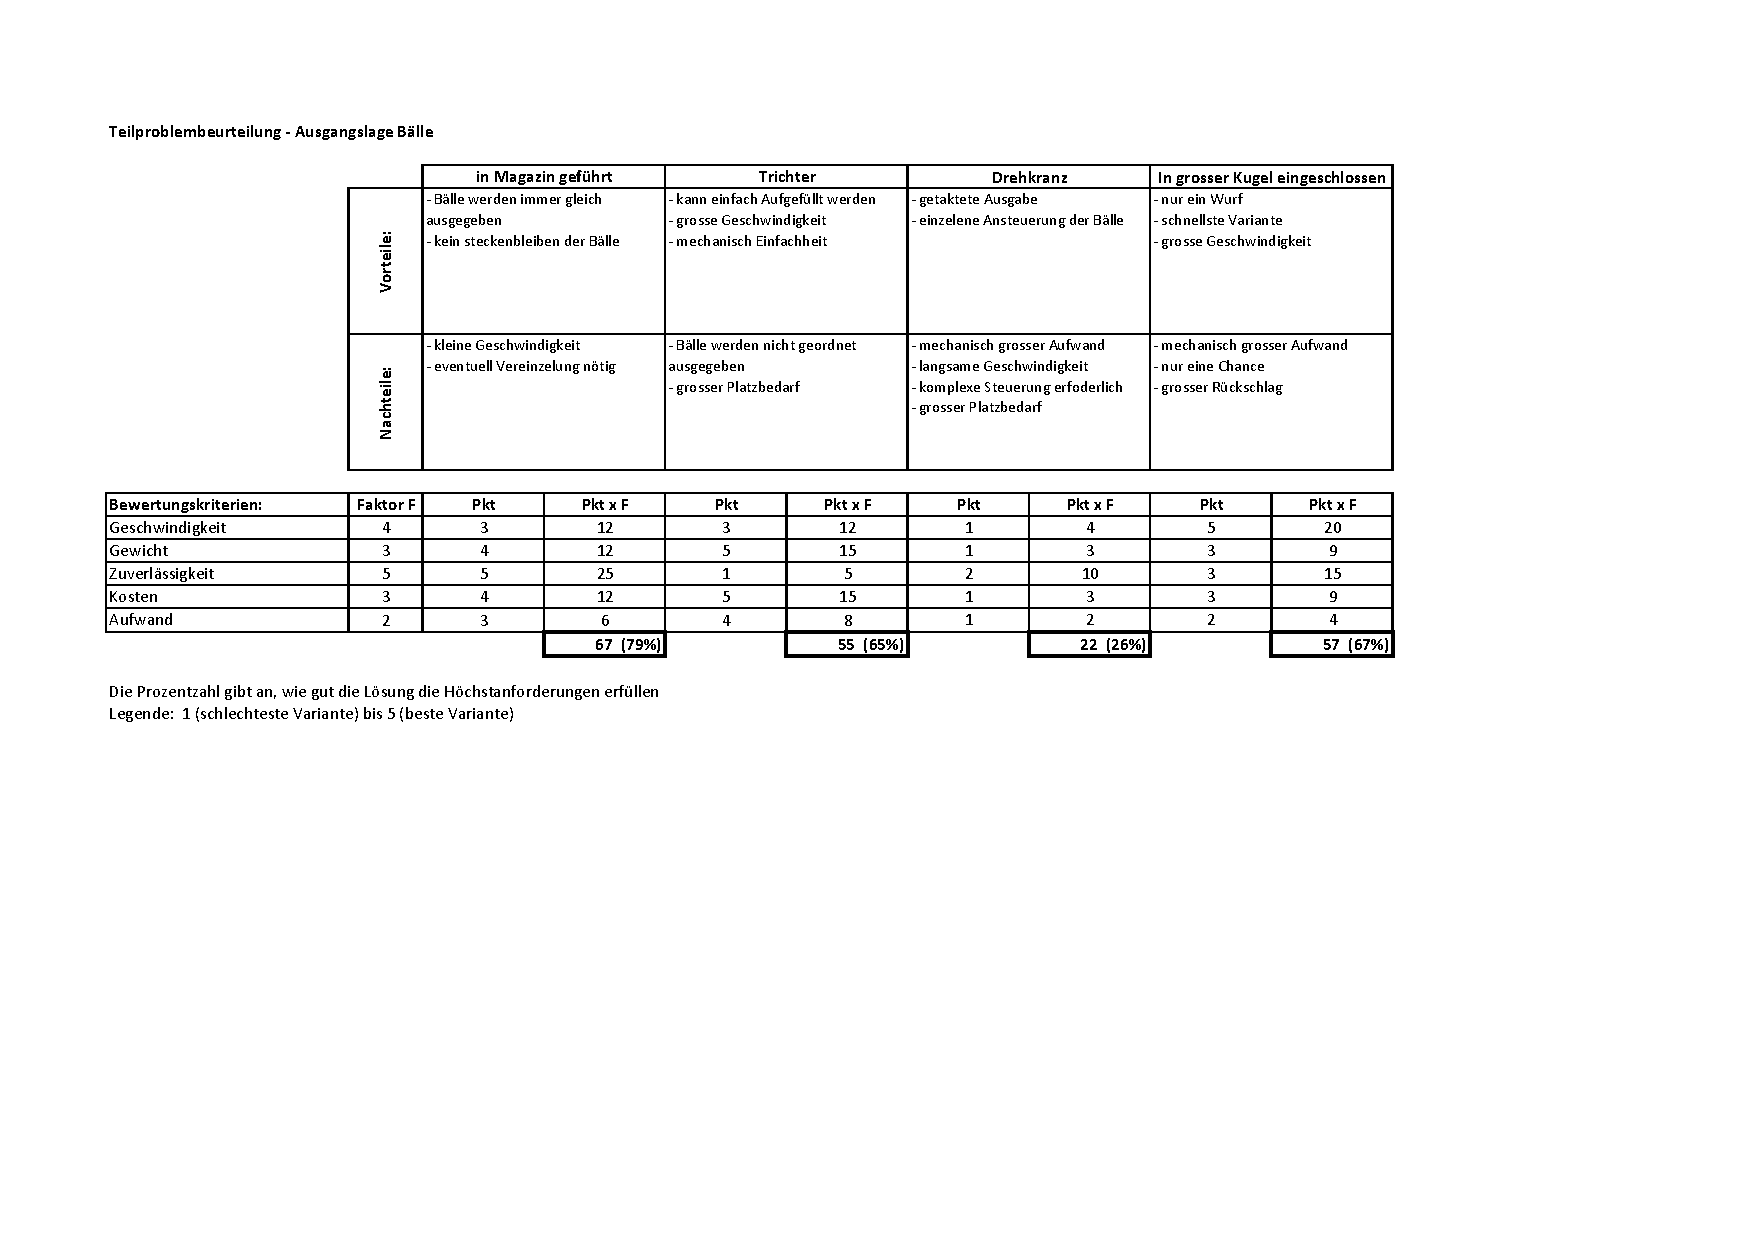
\includegraphics[page=1,scale=0.95,clip,trim=14mm 60mm 18mm 26mm] {Morphologie/Anhang/Teilproblembeurteilung-Ausgangslage_Baelle.pdf}
		\newpage
		\subsection{Startgerät-Endgerät}
		\label{apx:StartgeraetEndgeraet}
		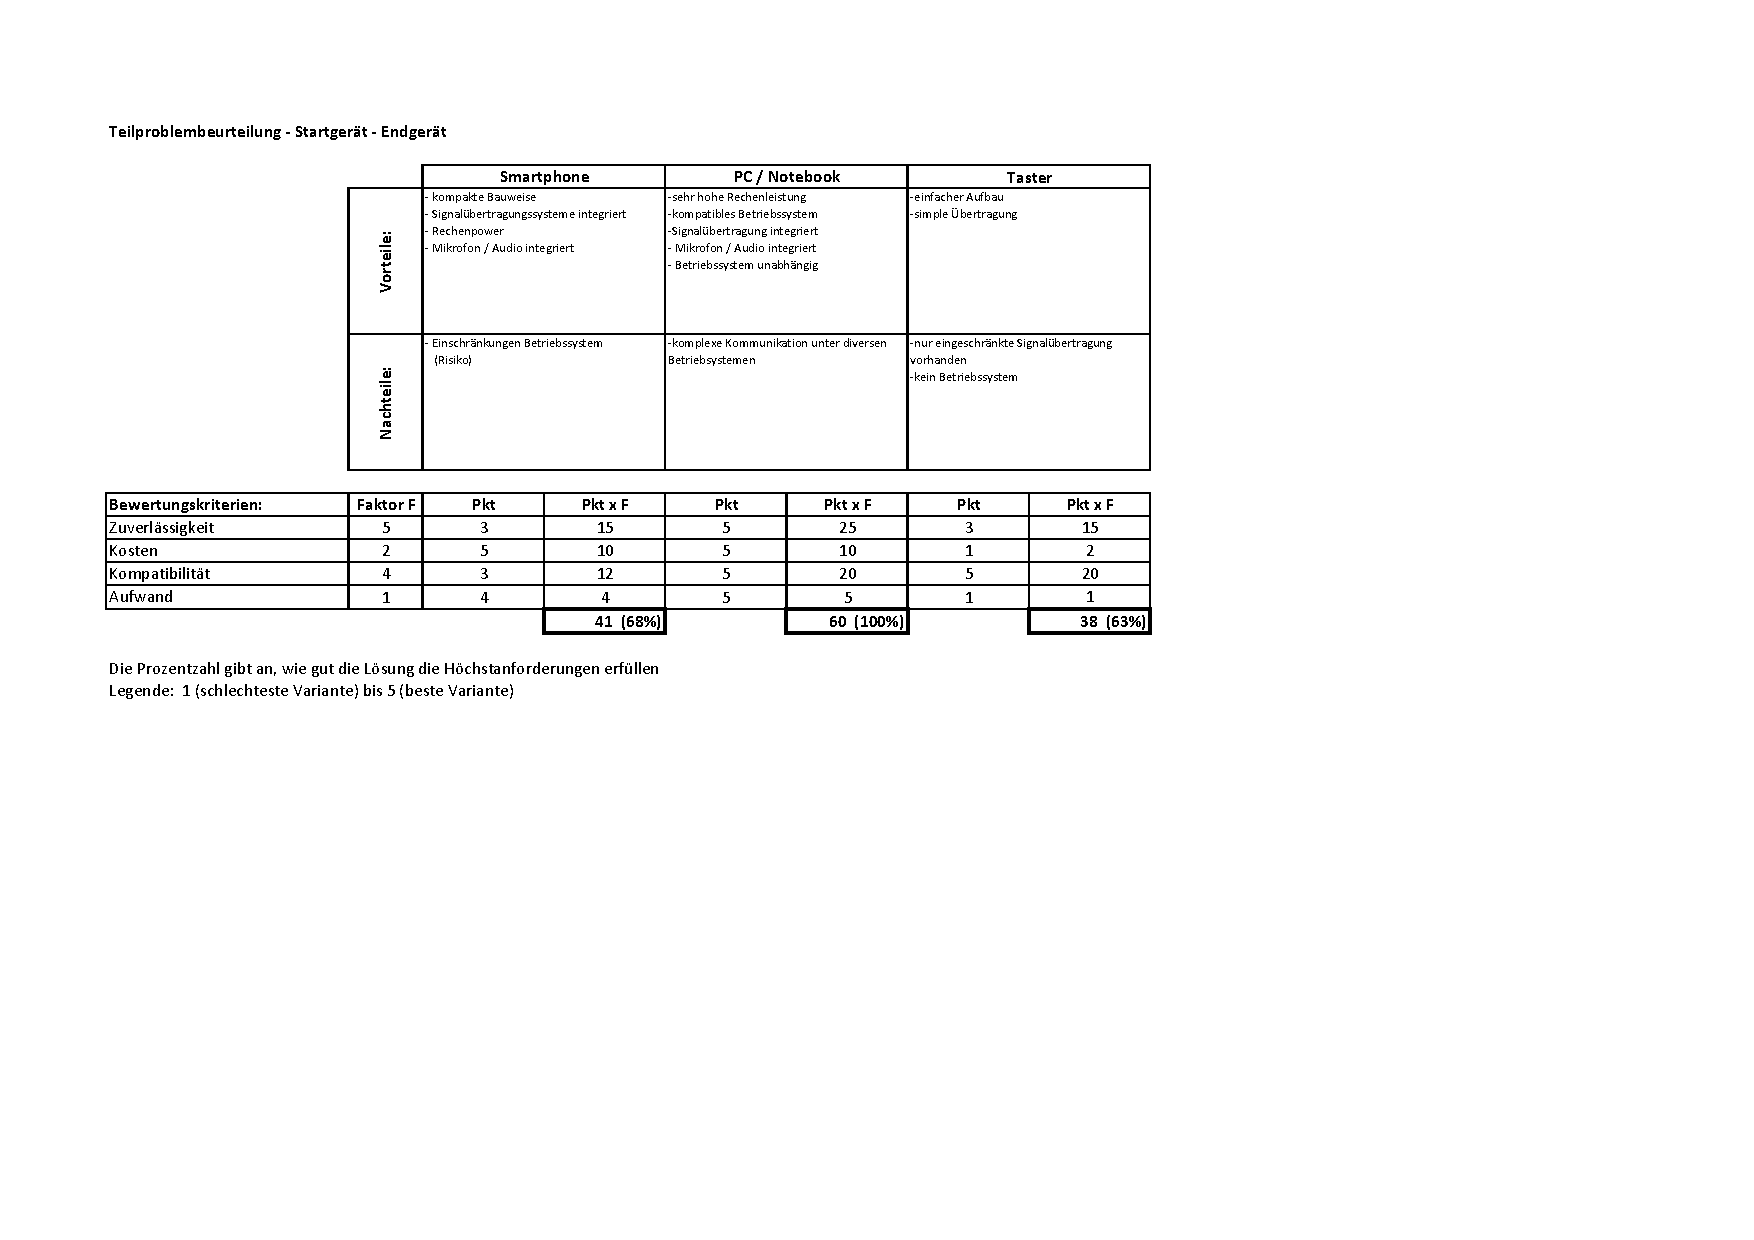
\includegraphics[page=1,scale=0.92,clip,trim=14mm 60mm 18mm 26mm] {Morphologie/Anhang/Teilproblembeurteilung-Startgeraet-Endgeraet.pdf}
		\newpage
		\subsection{Startbefehlübermittlung}
		
		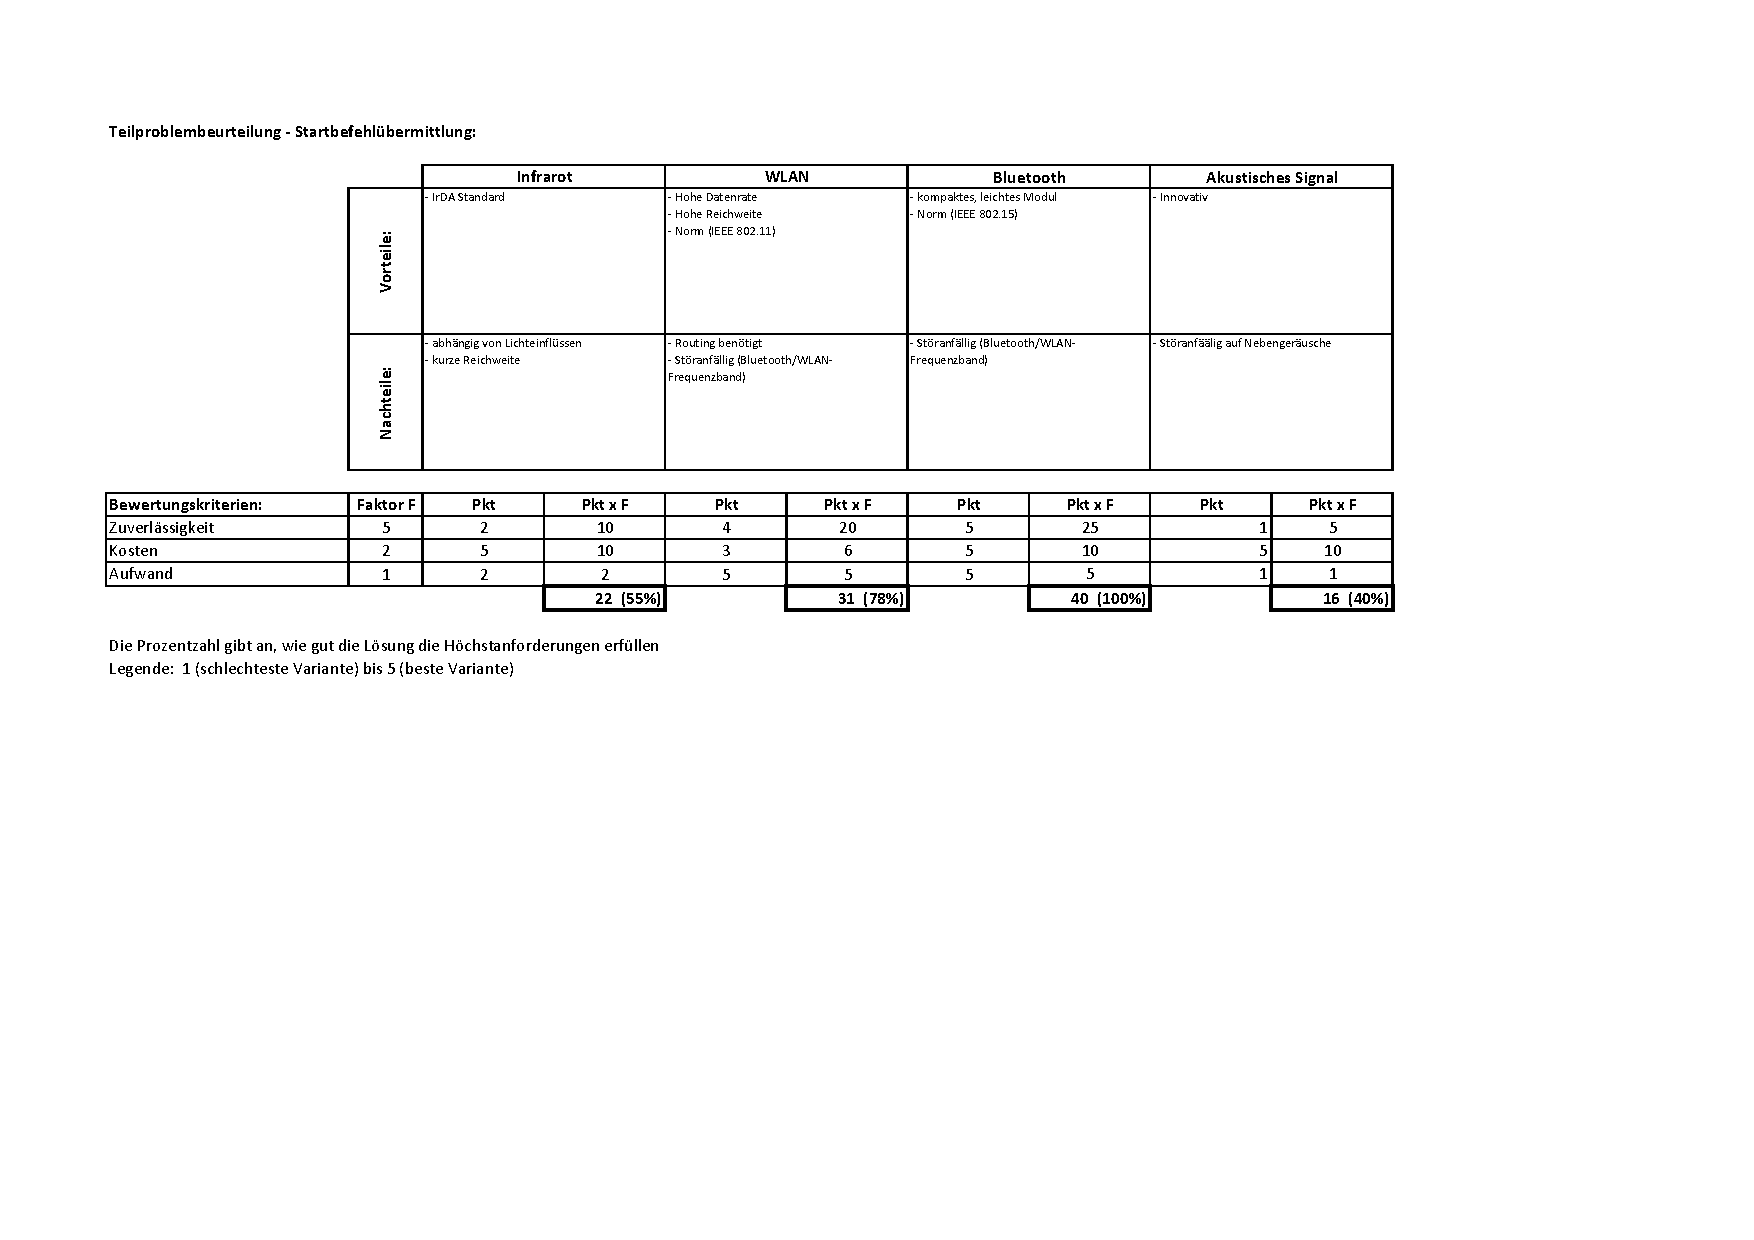
\includegraphics[page=1,scale=0.92,clip,trim=14mm 60mm 18mm 26mm] {Morphologie/Anhang/Teilproblembeurteilung-Startbefehluebermittlung.pdf}
		\newpage
		\subsection{Ausgangslage Rechnerkapazität}
		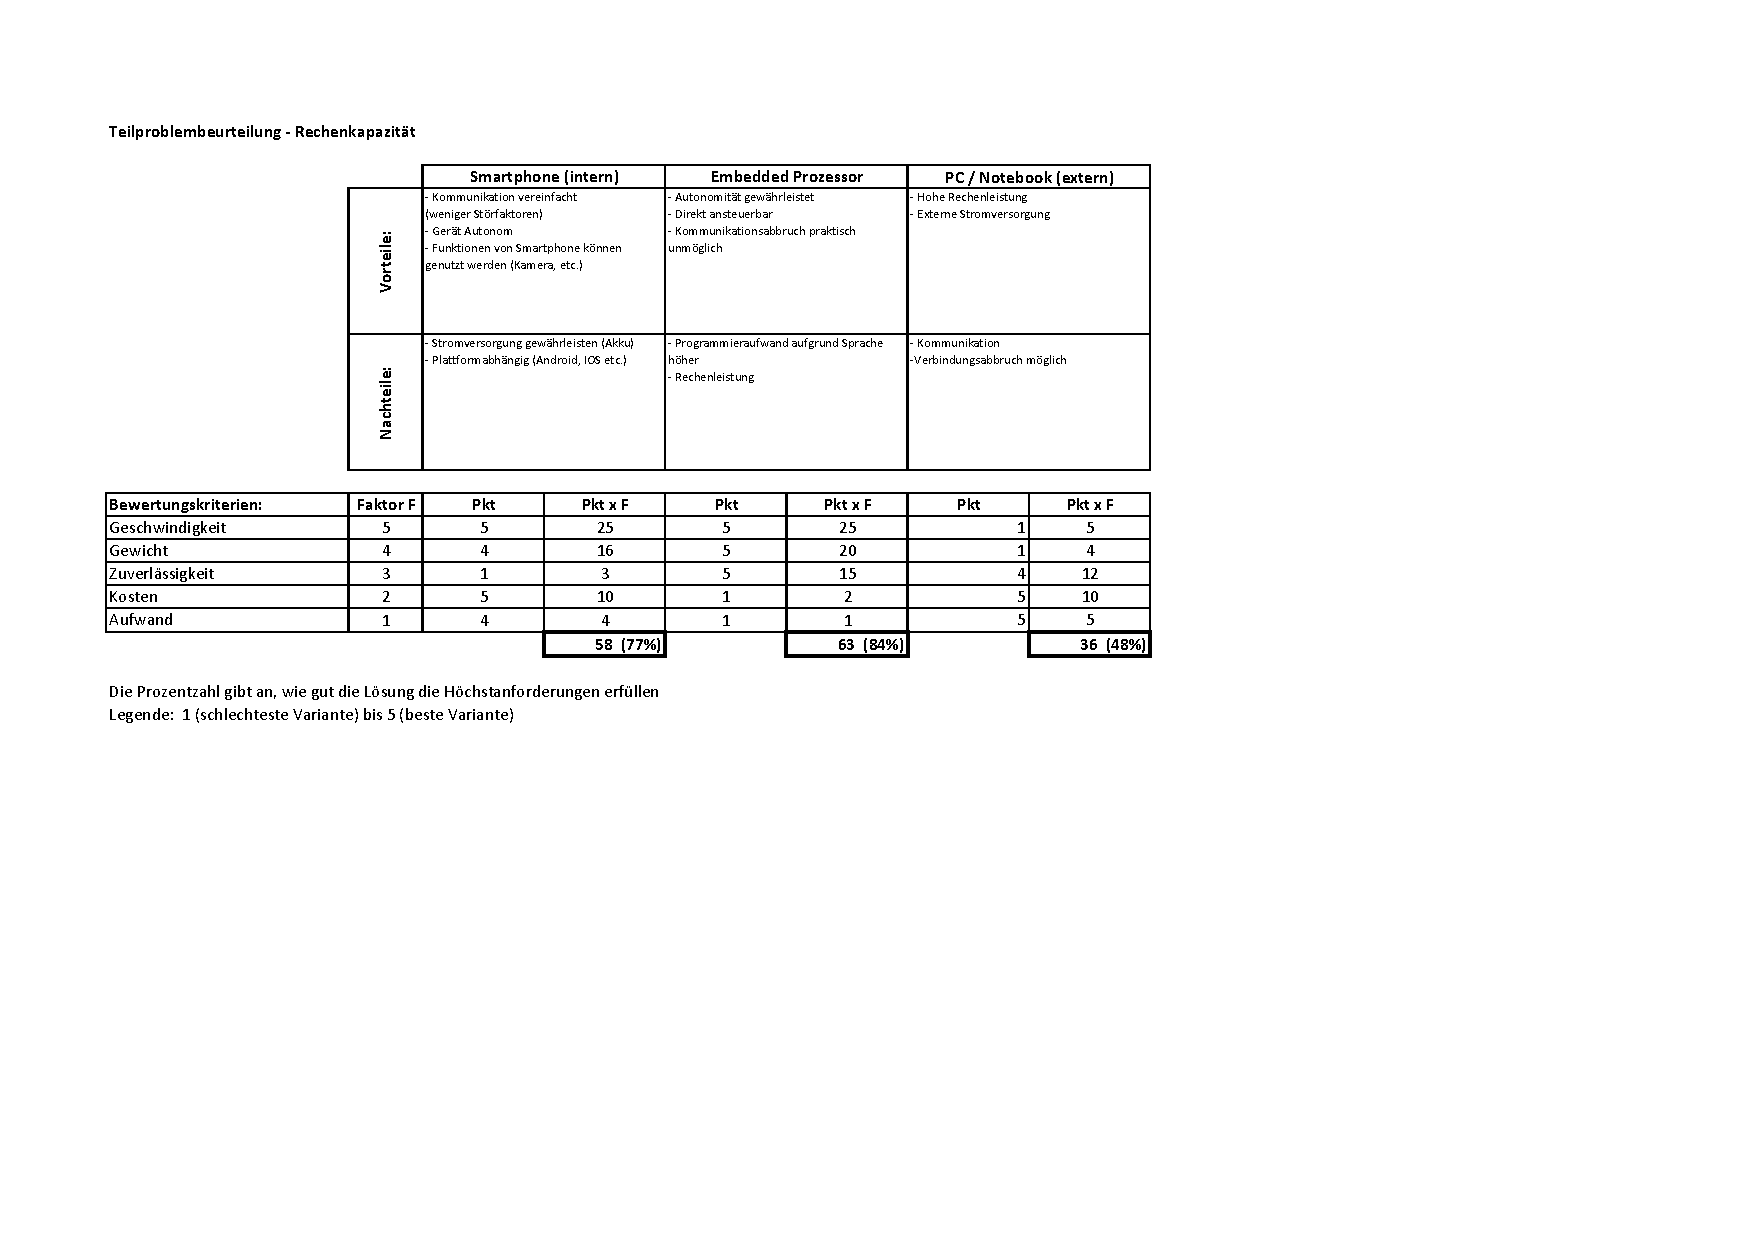
\includegraphics[page=1,scale=0.95,clip,trim=14mm 60mm 18mm 26mm] {Morphologie/Anhang/Teilproblembeurteilung-Rechenkapazitaet.pdf}
		\newpage
		\subsection{Versorgung und Steuerung}
		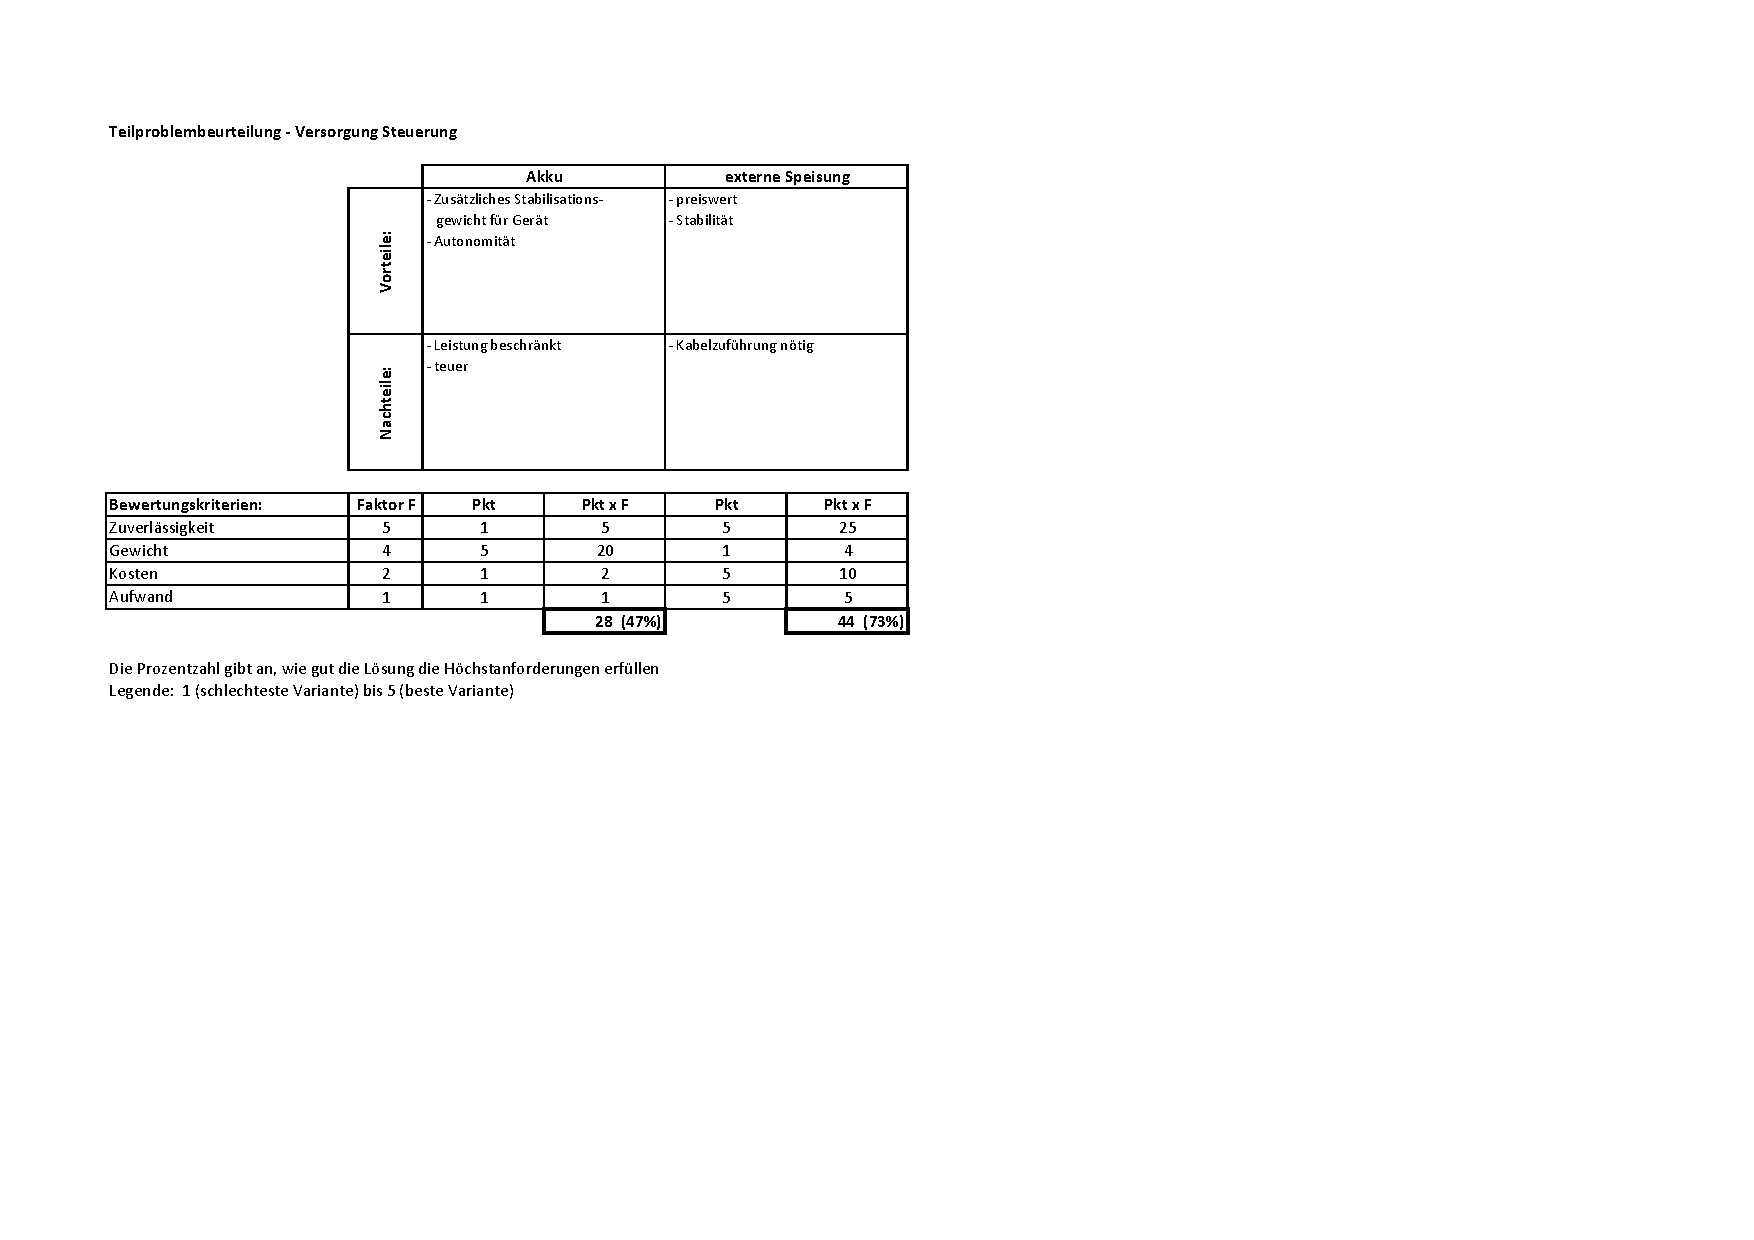
\includegraphics[page=1,scale=0.92,clip,trim=14mm 60mm 18mm 26mm] {Morphologie/Anhang/Teilproblembeurteilung-Versorgung_Steuerung.pdf}
		\newpage
		\subsection{Sensorik}
		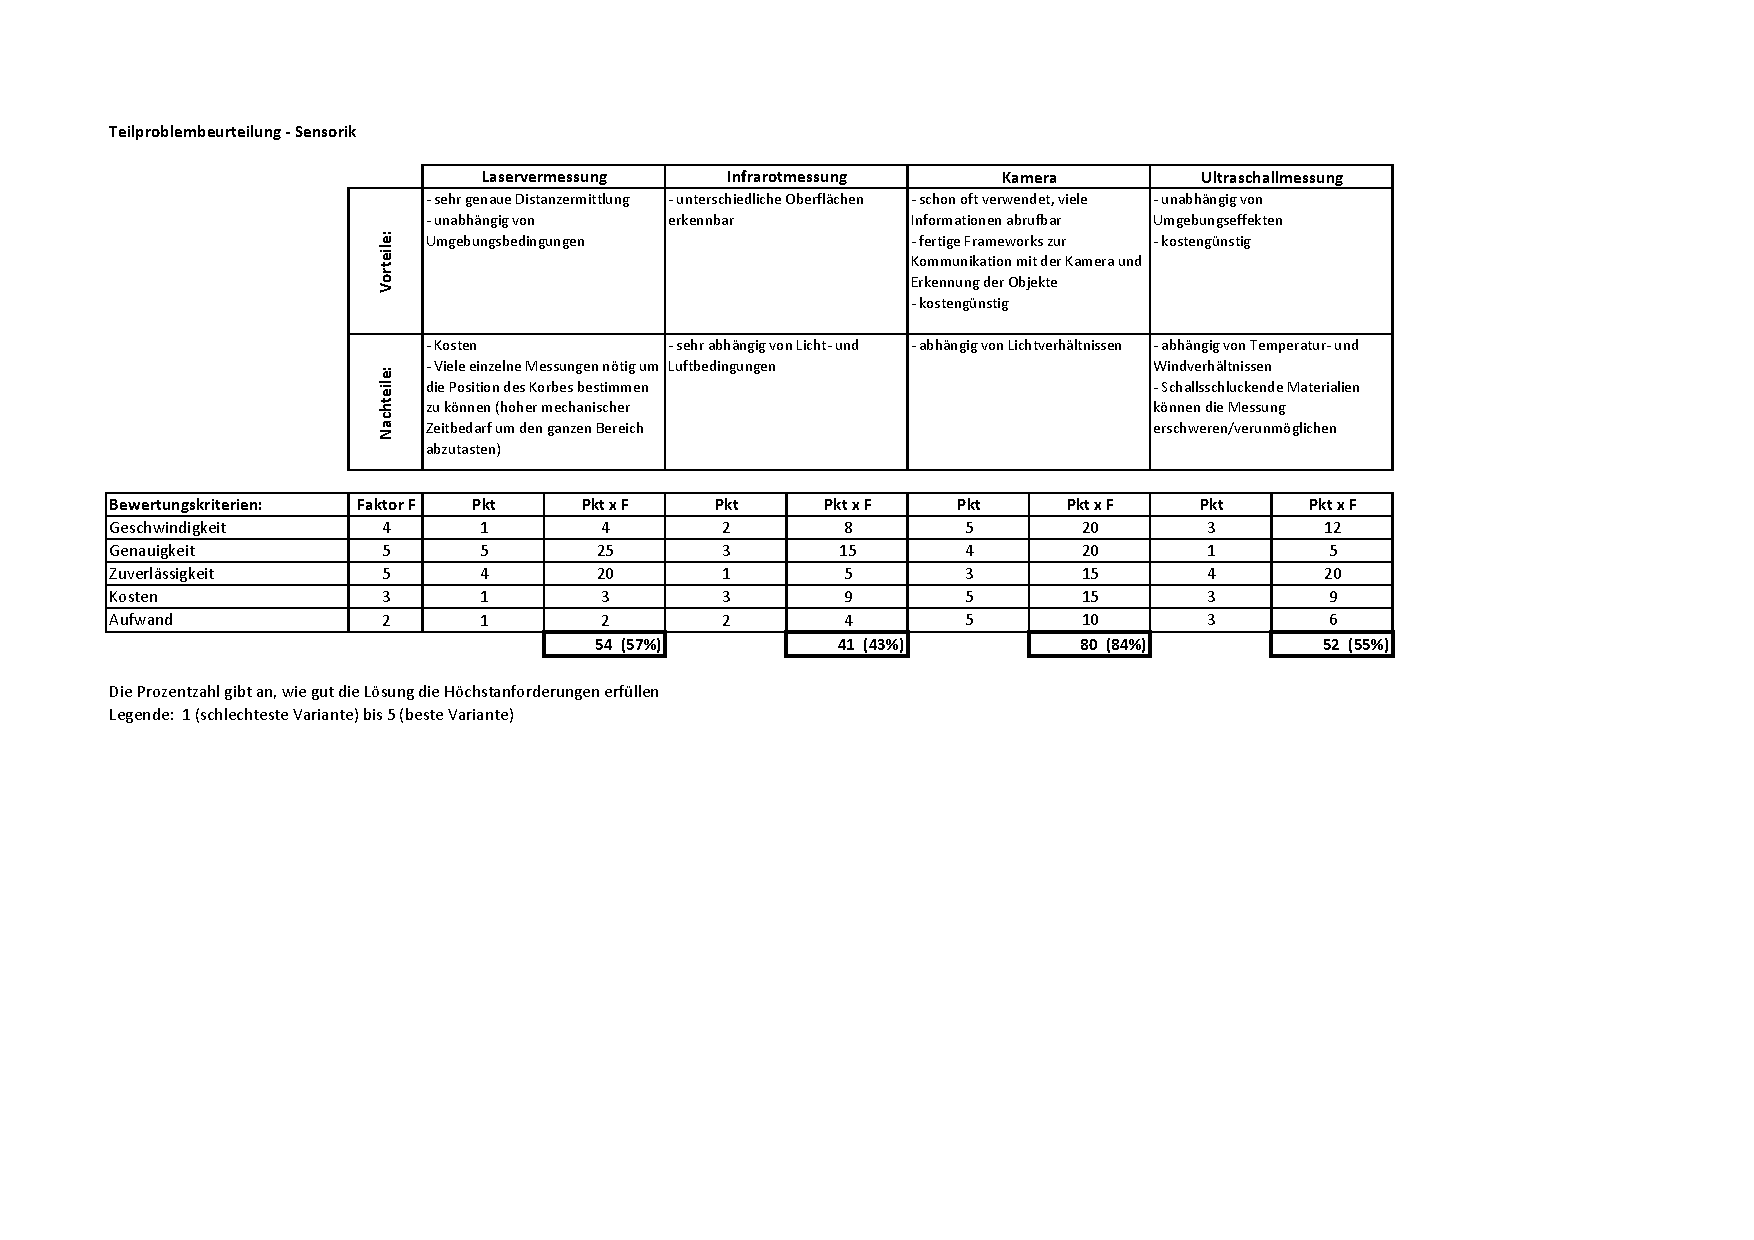
\includegraphics[page=1,scale=0.92,clip,trim=14mm 60mm 18mm 26mm] {Morphologie/Anhang/Teilproblembeurteilung-Sensorik.pdf}
		\newpage
		
		\subsection{Weg des Balles}
		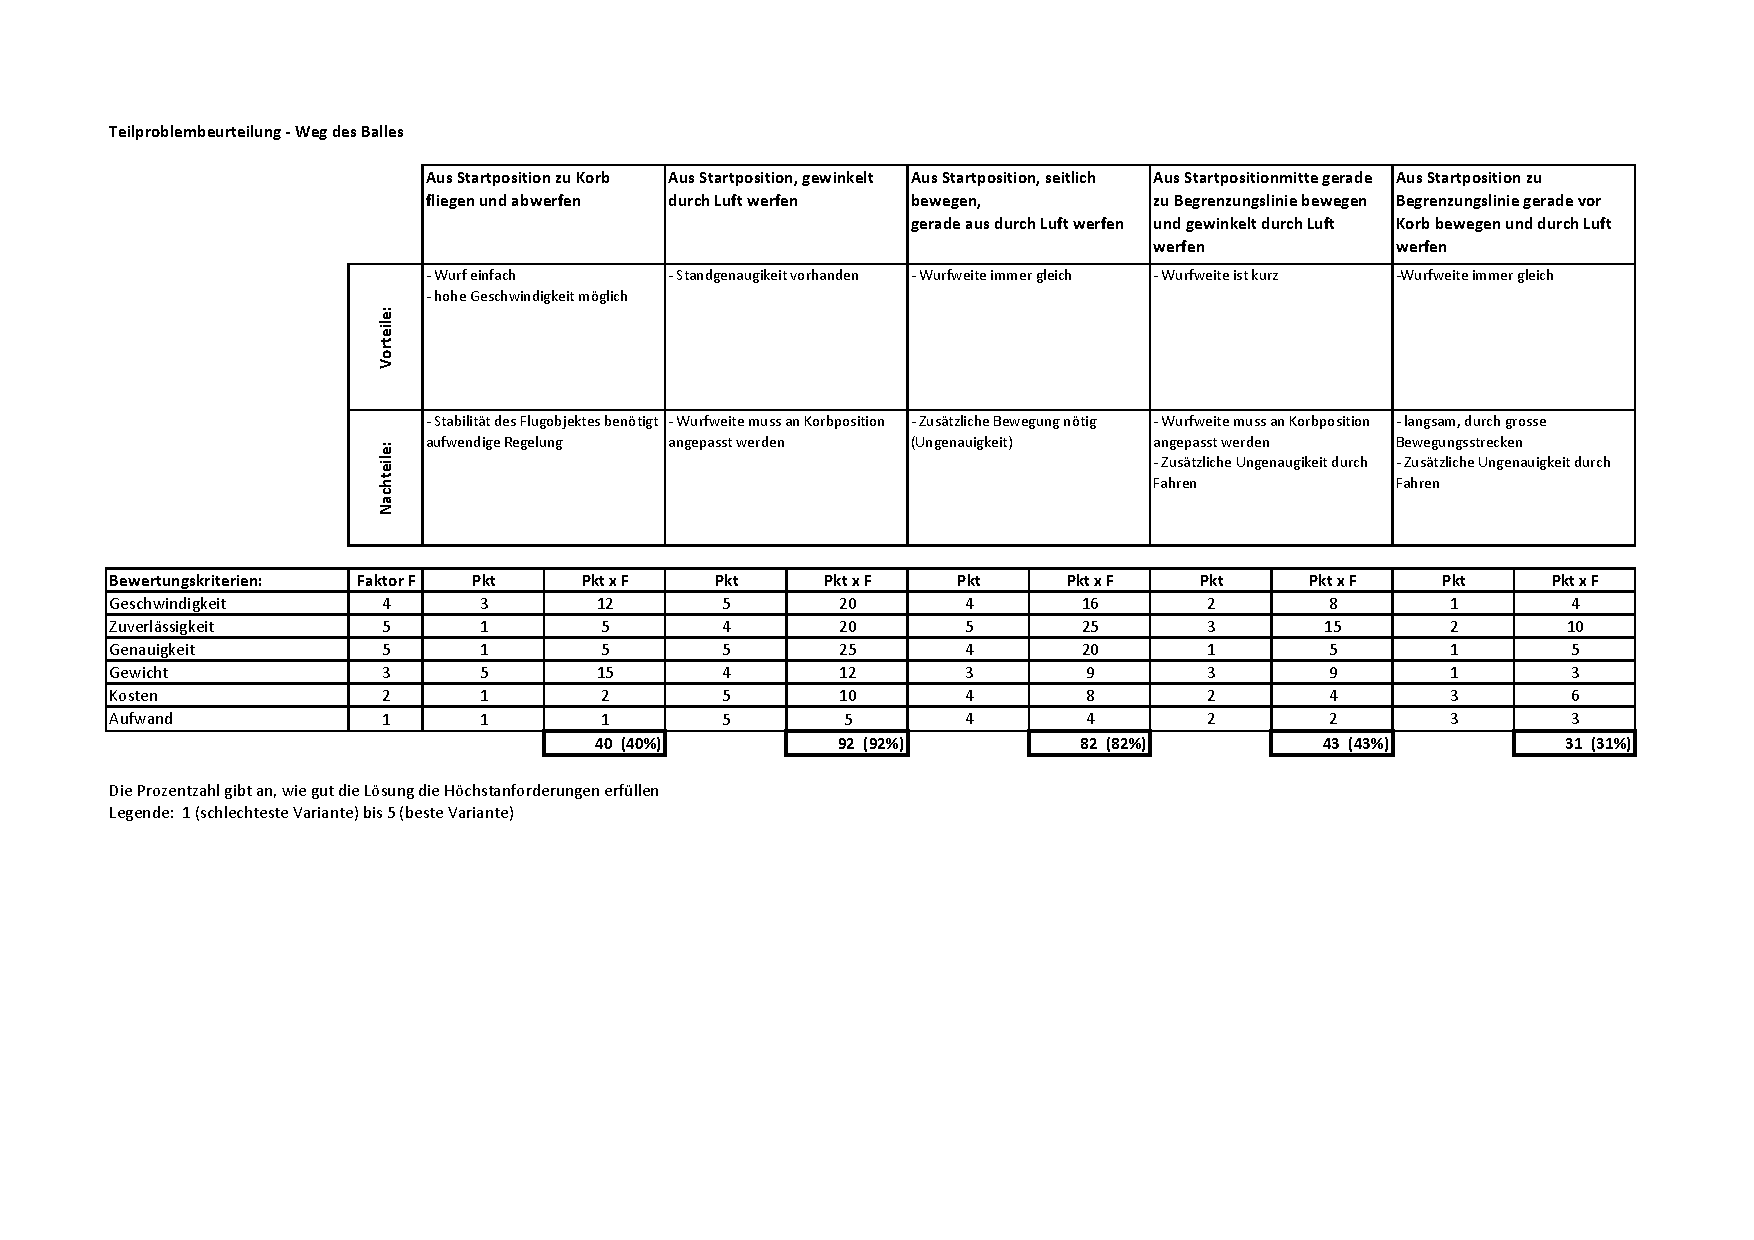
\includegraphics[page=1,scale=0.82,clip,trim=14mm 60mm 18mm 26mm] {Morphologie/Anhang/Teilproblembeurteilung-Weg_des_Balles.pdf}
\end{landscape} 
            \newpage
        \end{appendix} 
    
      
\end{document}